\documentclass[journal,twoside,web]{ieeecolor}
\usepackage{generic}
\usepackage{cite}
\usepackage{amsmath,amssymb,amsfonts}
\usepackage{algorithmic}
\usepackage{graphicx}
\usepackage{tikz}
\usetikzlibrary{arrows.meta,positioning}
\usepackage{booktabs}
\usepackage{algorithm,algorithmic}
\usepackage{hyperref}
\hypersetup{hidelinks}
\usepackage{textcomp}
\def\BibTeX{{\rm B\kern-.05em{\sc i\kern-.025em b}\kern-.08em
    T\kern-.1667em\lower.7ex\hbox{E}\kern-.125emX}}
\markboth{\hskip25pc IEEE TRANSACTIONS AND JOURNALS TEMPLATE}
{Author \MakeLowercase{\textit{et al.}}: Title}
\begin{document}
\title{Few-Shot Continual Learning for 3D Brain MRI with Frozen Foundation Models}

\author{Chi-Sheng Chen$^{1}$,
Xinyu Zhang$^{2}$,
En-Jui Kuo$^{5}$,
Rong Fu$^{2}$,
Qiuzhe Xie$^{3}$,
and Fan Zhang$^{4}$
\thanks{$^{1}$Beth Israel Deaconess Medical Center \& Harvard Medical School, Boston, MA 02115 USA.}
\thanks{$^{2}$Luddy School of Informatics, Computing, and Engineering, Indiana University Bloomington, Bloomington, IN 47405 USA.}
\thanks{$^{3}$Institute of Electronics Engineering, National Taiwan University, 106319, Taiwan.}
\thanks{$^{4}$Department of Mathematics, Boise State University, Boise, ID 83702 USA.}
\thanks{$^{5}$Department of Electrophysics, National Yang Ming Chiao Tung University, 30010, Taiwan.}}

\maketitle

\begin{abstract}
Foundation models pretrained on large-scale 3D medical imaging data face challenges when adapted to multiple downstream tasks under continual learning with limited labeled data. We address few-shot continual learning for 3D brain MRI by combining a frozen pretrained backbone with task-specific Low-Rank Adaptation (LoRA) modules. Tasks arrive sequentially---tumor segmentation (BraTS) and brain age estimation (IXI)---with no replay of previous task data. Each task receives a dedicated LoRA adapter; only the adapter and task-specific head are trained while the backbone remains frozen, thereby eliminating catastrophic forgetting by design (BWT=0). In continual learning, sequential full fine-tuning suffers severe forgetting (T1 Dice drops from 0.80 to 0.16 after T2), while sequential linear probing achieves strong T1 (Dice 0.79) but fails on T2 (MAE 1.45). Our LoRA approach achieves the best balanced performance across both tasks: T1 Dice 0.62$\pm$0.07, T2 MAE 0.16$\pm$0.05, with zero forgetting and $<$0.1\% trainable parameters per task, though with noted systematic age underestimation in T2 (Wilcoxon $p<0.001$). Frozen foundation models with task-specific LoRA adapters thus offer a practical solution when both tasks must be maintained under few-shot continual learning.
\end{abstract}

\begin{IEEEkeywords}
Few-shot learning \and Continual learning \and LoRA \and 3D brain MRI \and Foundation models \and Parameter-efficient fine-tuning.
\end{IEEEkeywords}

\section{Introduction}
\label{sec:introduction}
% \IEEEPARstart{T}{his} document is a template for \LaTeX. \section{Introduction}

\IEEEPARstart{M}{edical} imaging AI increasingly relies on foundation models pretrained on large-scale datasets~\cite{fomo2025,baseline}. \label{sec:intro}
When deployed in clinical settings, these models must adapt to multiple tasks---e.g., tumor segmentation and brain age estimation---often with limited labeled data and without access to prior task samples due to privacy or storage constraints. In practice, radiology departments may introduce new analysis tasks over time (e.g., adding brain age prediction to an existing tumor workflow) with only a small batch of newly annotated cases. This scenario motivates \emph{few-shot continual learning}: learning new tasks sequentially from few examples while retaining performance on previously learned tasks.

Sequential fine-tuning of shared backbone parameters typically causes \emph{catastrophic forgetting}~\cite{kirkpatrick2017,mccloskey1989catastrophic}: when the model is updated for a new task, performance on prior tasks degrades sharply. Existing continual learning strategies such as EWC~\cite{kirkpatrick2017} and LwF~\cite{li2017lwf} mitigate forgetting by regularizing or distilling, but require careful tuning and may still overwrite critical representations. An alternative is to \emph{freeze} the pretrained backbone and adapt only small task-specific modules. Parameter-efficient fine-tuning methods such as LoRA~\cite{hu2022lora, hu2024computational} inject low-rank matrices into selected layers, training a small fraction of parameters while preserving the original weights.

We propose a continual learning framework for 3D brain MRI that combines a frozen FOMO-style pretrained backbone~\cite{fomo2025} with task-specific LoRA adapters. Tasks arrive sequentially; each task receives its own LoRA module and task head. No replay buffer or access to previous-task data is required. Because the backbone and prior adapters remain frozen when training a new task, catastrophic forgetting is eliminated by design: BWT is identically zero.

We evaluate on two downstream tasks using public datasets: tumor segmentation (BraTS 2023 Glioma) and brain age estimation (IXI). We compare against sequential linear probing (frozen backbone, train heads only) and sequential full fine-tuning. The key finding is that \emph{only LoRA maintains balanced performance across both tasks} in the continual setting:
\begin{itemize}
\item \textbf{Sequential FT} achieves high T1 Dice (0.80) and T2 MAE (0.004$^*$) during training, but suffers severe forgetting: T1 Dice collapses to 0.16 after T2 (BWT$\approx$-0.65). $^*$T2 MAE likely overfits on few-shot validation.
\item \textbf{Sequential Linear} achieves strong T1 (Dice 0.79) with mild forgetting (BWT$\approx$-0.01), but \emph{fails on T2} (MAE 1.45).
\item \textbf{LoRA} attains T1 Dice 0.62$\pm$0.07, T2 MAE 0.16$\pm$0.05, BWT=0, with $<$0.1\% trainable params per task---the only method that maintains reasonable performance on both tasks without forgetting.
\end{itemize}

Our contributions are: (1) a continual learning formulation using frozen backbones and task-specific LoRA for 3D brain MRI; (2) empirical validation on BraTS and IXI showing LoRA achieves best balanced performance; and (3) ablations on LoRA placement and shot count.


\section{Related Work}
\label{sec:related}

\subsection{Foundation Models for Medical Imaging}

Large-scale pretrained models have transformed medical image analysis. The FOMO initiative~\cite{fomo2025} provides 3D foundation models pretrained on diverse medical imaging datasets via masked autoencoding objectives, yielding general-purpose representations for downstream adaptation. UNETR~\cite{unetr} introduced Vision Transformers into 3D medical segmentation by replacing CNN encoders with self-attention, demonstrating strong performance on multi-organ and brain tumor segmentation. More recently, SAM-Med3D~\cite{sammed3d} extended the Segment Anything paradigm to volumetric data, and domain-specific foundation models have emerged for pathology~\cite{chen2024towards} and radiology. These models share a common deployment challenge: adapting to multiple downstream tasks efficiently while preserving the pretrained representations, particularly when labeled data is scarce.

\subsection{Continual Learning in Medical Imaging}

Continual learning addresses the problem of sequentially learning new tasks without forgetting previously acquired knowledge~\cite{mccloskey1989catastrophic}. Classical approaches fall into three categories: (i)~\emph{regularization-based} methods such as EWC~\cite{kirkpatrick2017} and Synaptic Intelligence~\cite{zenke2017continual}, which penalize changes to important parameters; (ii)~\emph{replay-based} methods such as iCaRL~\cite{rebuffi2017icarl}, which store or generate exemplars from prior tasks; and (iii)~\emph{distillation-based} methods such as LwF~\cite{li2017lwf}, which use the previous model's outputs as soft targets. In medical imaging, continual learning has been explored primarily for class-incremental segmentation: LifeLonger~\cite{derakhshani2022lifelonger} benchmarks continual disease classification across dermatology datasets, while Lifelong nnU-Net~\cite{gonzalez2023lifelong} standardizes continual organ segmentation. However, most prior work considers \emph{class-incremental} settings with homogeneous outputs (e.g., adding new organ classes). Our work addresses \emph{task-incremental} continual learning across \emph{heterogeneous} output types---segmentation and regression---which presents distinct challenges since the task heads and loss functions differ fundamentally.

\subsection{Parameter-Efficient Fine-Tuning}

Parameter-efficient fine-tuning (PEFT) methods adapt large pretrained models by training only a small subset of parameters. LoRA~\cite{hu2022lora} injects trainable low-rank decompositions into weight matrices, achieving competitive performance with full fine-tuning at a fraction of the parameter cost. Alternative PEFT approaches include Adapters~\cite{houlsby2019}, which insert bottleneck modules between layers; Prefix-Tuning~\cite{prefix_tuning}, which prepends learnable tokens to the input; and BitFit~\cite{bitfit}, which tunes only bias terms. In the context of continual learning, PEFT methods offer a natural mechanism for task isolation: PackNet~\cite{packnet} iteratively prunes and freezes network capacity per task, while Piggyback~\cite{piggyback} learns binary masks over a shared backbone. Our approach is most closely related to adapter-isolation strategies but leverages LoRA's low-rank structure for 3D convolutions, which is more parameter-efficient than full adapter layers and directly compatible with pretrained UNet architectures.


\section{Method}
\label{sec:method}

\subsection{Problem Formulation}
\label{sec:problem}

We consider continual learning with sequential task arrival. Let $f_\theta$ denote a pretrained 3D UNet backbone (frozen) and $\mathcal{T}_1, \mathcal{T}_2, \ldots, \mathcal{T}_K$ a sequence of tasks. For each task $k$, we have access to only $N_k \in \{16, 32, 64\}$ labeled few-shot samples drawn from task-specific distribution $\mathcal{D}_k = \{(x_i^{(k)}, y_i^{(k)})\}_{i=1}^{N_k}$. We assume \emph{no replay}: when training on $\mathcal{T}_k$, we cannot access data from $\mathcal{T}_{<k}$. The optimization objective for task $k$ is:
\begin{equation}
\min_{\phi_k, h_k} \; \frac{1}{N_k} \sum_{i=1}^{N_k} \mathcal{L}_k \bigl( h_k(f_\theta(x_i^{(k)}; \phi_k)),\; y_i^{(k)} \bigr)
\label{eq:objective}
\end{equation}
where $\phi_k$ denotes the LoRA adapter parameters for task $k$, $h_k$ the task-specific head, and $\mathcal{L}_k$ the task loss. Crucially, $\theta$ remains frozen throughout; only $\phi_k$ and $h_k$ are optimized. The goal is to learn $\{\phi_k, h_k\}_{k=1}^K$ such that performance on all seen tasks remains high after training on $\mathcal{T}_K$.

We evaluate two tasks: (1) tumor segmentation (3D binary mask) and (2) brain age estimation (regression). Each task has modality-specific inputs (BraTS: T2w, T2-FLAIR, T1c; IXI: T1, T2) and a distinct output head $h_k$.

Figure~\ref{fig:framework} illustrates the overall pipeline: a frozen pretrained backbone, task-specific LoRA adapters, and task heads. At inference for task $k$, we use backbone $f_\theta$ + adapter $\phi_k$ + head $h_k$; prior adapters and the backbone remain frozen.

\begin{figure*}[t]
\centering
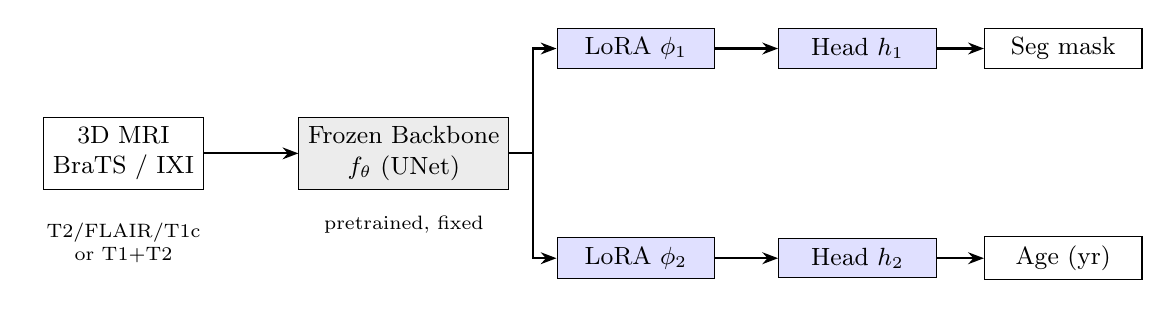
\begin{tikzpicture}[
  node distance=0.5cm and 0.8cm,
  box/.style={draw, minimum width=2cm, minimum height=0.5cm, align=center, font=\small},
  bigbox/.style={draw, minimum width=2.2cm, minimum height=0.7cm, align=center, font=\small},
  frozen/.style={fill=gray!15, box},
  trainable/.style={fill=blue!12, box},
  arrow/.style={-{Stealth[length=2mm]}, thick}
]
  \node[box] (input) {3D MRI\\BraTS / IXI};
  \node[below=0.3cm of input, font=\scriptsize, text width=2.2cm, align=center] {T2/FLAIR/T1c or T1+T2};
  \node[bigbox, frozen, right=1.2cm of input] (backbone) {Frozen Backbone\\$f_\theta$ (UNet)};
  \node[below=0.2cm of backbone, font=\scriptsize] {pretrained, fixed};
  \node[box, trainable, above right=0.6cm and 0.6cm of backbone] (lora1) {LoRA $\phi_1$};
  \node[box, trainable, below right=0.6cm and 0.6cm of backbone] (lora2) {LoRA $\phi_2$};
  \node[box, trainable, right=0.8cm of lora1] (head1) {Head $h_1$};
  \node[box, trainable, right=0.8cm of lora2] (head2) {Head $h_2$};
  \node[box, right=0.6cm of head1] (out1) {Seg mask};
  \node[box, right=0.6cm of head2] (out2) {Age (yr)};
  \draw[arrow] (input) -- (backbone);
  \draw[arrow] (backbone.east) -- ++(0.3,0) |- (lora1.west);
  \draw[arrow] (backbone.east) -- ++(0.3,0) |- (lora2.west);
  \draw[arrow] (lora1) -- (head1);
  \draw[arrow] (lora2) -- (head2);
  \draw[arrow] (head1) -- (out1);
  \draw[arrow] (head2) -- (out2);
\end{tikzpicture}
\caption{Framework: frozen pretrained backbone $f_\theta$ with task-specific LoRA adapters $\phi_k$ and heads $h_k$. Gray = frozen; blue = trainable per task. At inference for T1 (resp.\ T2): backbone + $\phi_1$ + $h_1$ (resp.\ $\phi_2$ + $h_2$).}
\label{fig:framework}
\end{figure*}

\subsection{LoRA for 3D Convolutions}
\label{sec:lora}

Low-Rank Adaptation (LoRA)~\cite{hu2022lora} injects trainable low-rank matrices into a frozen weight matrix $W \in \mathbb{R}^{d \times k}$:
\begin{equation}
W' = W + \Delta W, \quad \Delta W = \frac{\alpha}{r} B \cdot A, \quad A \in \mathbb{R}^{r \times k}, \; B \in \mathbb{R}^{d \times r}
\label{eq:lora}
\end{equation}
with rank $r \ll \min(d,k)$ and scaling factor $\alpha$. Only $A$ and $B$ are trained; $W$ stays frozen. The scaling ratio $\alpha/r$ controls the magnitude of the low-rank perturbation relative to the pretrained weights.

For 3D convolutions in a UNet, we reshape the Conv3d weight tensor $W \in \mathbb{R}^{C_{\text{out}} \times C_{\text{in}} \times D \times H \times W}$ and apply LoRA via parallel $1\times1\times1$ convolutions acting on the channel dimension:
\begin{equation}
\text{Conv3d}'(x) = \text{Conv3d}(x; W) + \frac{\alpha}{r} \, \text{Conv1}(x; B) \circ \text{Conv1}(x; A)
\label{eq:lora3d}
\end{equation}
where Conv1 denotes $1\times1\times1$ convolution, $A \in \mathbb{R}^{r \times C_{\text{in}}}$ projects to rank-$r$ space, and $B \in \mathbb{R}^{C_{\text{out}} \times r}$ projects back. This formulation is memory-efficient and compatible with standard Conv3d layers~\cite{peft}.

We use rank $r \in \{4, 8, 16\}$ (default $r=8$), $\alpha=16$, and target both encoder and decoder blocks for segmentation; encoder-only suffices for classification and regression. For a single Conv3d layer with input channels $C_{\text{in}}$ and output channels $C_{\text{out}}$, the number of LoRA parameters is:
\begin{equation}
|\phi_{\text{layer}}| = r \cdot (C_{\text{in}} + C_{\text{out}})
\label{eq:param_count}
\end{equation}
which is substantially smaller than the original $C_{\text{out}} \times C_{\text{in}} \times D \times H \times W$ parameters. Summing over all targeted layers, the total LoRA parameters per task satisfy $|\phi_k| \ll |\theta|$, yielding $<$0.1\% trainable parameters relative to the backbone ($\sim$50M params).

\subsection{Continual Learning via Adapter Isolation}
\label{sec:continual}

Each task $k$ receives a \emph{dedicated LoRA adapter} $\phi_k$. The full training and inference procedure is summarized in Algorithm~\ref{alg:continual}. The trainable parameter set for task $k$ is strictly disjoint from all other tasks:
\begin{equation}
\Phi_k = \{\phi_k, h_k\}, \quad \Phi_i \cap \Phi_j = \emptyset \;\; \forall \, i \neq j
\label{eq:disjoint}
\end{equation}
Because $\theta$ and $\{\Phi_{<k}\}$ are frozen when optimizing $\Phi_k$, the performance of any prior task $j < k$ is invariant to training on $\mathcal{T}_k$. Formally, let $R_{t,j}$ denote the performance of task $j$ after training up to task $t$. Then:
\begin{equation}
R_{t,j} = R_{j,j} \quad \forall \, t \geq j \implies \text{BWT}_j = R_{K,j} - R_{j,j} = 0
\label{eq:bwt_zero}
\end{equation}
This zero-forgetting guarantee holds \emph{by construction}, without requiring any regularization or replay mechanism. At inference for task $k$, we simply load backbone $f_\theta$ + adapter $\phi_k$ + head $h_k$; no shared adapter exists across tasks. The total model storage after $K$ tasks is:
\begin{equation}
\text{Storage} = |\theta| + \sum_{k=1}^{K} (|\phi_k| + |h_k|)
\label{eq:storage}
\end{equation}
which grows linearly in $K$ but with a very small per-task overhead since $|\phi_k| \ll |\theta|$.

\begin{algorithm}[t]
\caption{Continual Learning via LoRA Adapter Isolation}
\label{alg:continual}
\begin{algorithmic}[1]
\REQUIRE Pretrained backbone $f_\theta$; task sequence $\mathcal{T}_1, \ldots, \mathcal{T}_K$; few-shot datasets $\mathcal{D}_1, \ldots, \mathcal{D}_K$ with $|\mathcal{D}_k| = N_k$; LoRA rank $r$; epochs $E$
\ENSURE Trained adapters $\{\phi_k\}_{k=1}^K$ and heads $\{h_k\}_{k=1}^K$
\STATE Freeze all parameters of $f_\theta$
\FOR{$k = 1$ \TO $K$}
    \STATE Initialize LoRA adapter $\phi_k$ with rank $r$ (random $A$, zero $B$)
    \STATE Initialize task head $h_k$ (decoder for segmentation, regressor for regression)
    \IF{$k > 1$}
        \STATE Freeze all previous adapters $\phi_1, \ldots, \phi_{k-1}$ and heads $h_1, \ldots, h_{k-1}$
    \ENDIF
    \STATE Split $\mathcal{D}_k$ into train/val sets (80\%/20\%)
    \FOR{epoch $= 1$ \TO $E$}
        \FOR{each mini-batch $(x, y) \in \mathcal{D}_k^{\text{train}}$}
            \STATE $\hat{y} \leftarrow h_k(f_\theta(x; \phi_k))$ \COMMENT{Forward with frozen backbone + active LoRA}
            \STATE Compute loss: $\mathcal{L}_k(\hat{y}, y)$ \COMMENT{Dice+BCE for seg; MSE for reg}
            \STATE Update only $\phi_k, h_k$ via Adam: $(\phi_k, h_k) \leftarrow (\phi_k, h_k) - \eta \nabla_{(\phi_k, h_k)} \mathcal{L}_k$
        \ENDFOR
    \ENDFOR
    \STATE Save $\phi_k, h_k$ to disk
\ENDFOR
\STATE \textbf{Inference for task $k$:} Load $f_\theta$, $\phi_k$, $h_k$; predict $\hat{y} = h_k(f_\theta(x; \phi_k))$
\end{algorithmic}
\end{algorithm}

\subsection{Task Heads and Losses}
\label{sec:heads}

Each task uses a dedicated output head and loss function matched to its output type.

\textbf{Task 1 (Segmentation).} The full UNet decoder produces a voxel-wise binary prediction. We apply LoRA to both encoder and decoder blocks, as the decoder must generate spatially detailed masks. The training loss combines Dice loss and binary cross-entropy (BCE):
\begin{equation}
\mathcal{L}_{\text{seg}} = 1 - \frac{2 \sum_i p_i g_i + \epsilon}{\sum_i p_i + \sum_i g_i + \epsilon} + \text{BCE}(p, g)
\end{equation}
where $p_i$ and $g_i$ denote predicted and ground-truth voxel values, and $\epsilon=10^{-5}$ ensures numerical stability. The Dice term directly optimizes overlap, while BCE provides voxel-level gradient signal that stabilizes training in few-shot regimes where foreground-background imbalance is severe.

\textbf{Task 2 (Regression).} For brain age estimation, we use an encoder-only architecture: features from the frozen encoder (with LoRA) are passed through global average pooling (GAP) followed by a two-layer fully connected head (ClsRegHead) with a single scalar output. Only encoder LoRA is applied since no spatial decoder is needed. The loss is mean squared error:
\begin{equation}
\mathcal{L}_{\text{reg}} = \frac{1}{N} \sum_{i=1}^{N} (\hat{y}_i - y_i)^2
\end{equation}
where $\hat{y}_i$ is the predicted age and $y_i$ the ground-truth age in years.

Training uses the Adam optimizer with a fixed learning rate of $10^{-3}$ and per-channel Z-score normalization. Patch size is $64\times64\times64$ for all continual experiments. No learning rate scheduling or early stopping is applied; we train for a fixed number of epochs to maintain consistency across methods and seeds.

\section{Experiments}
\label{sec:experiments}

\subsection{Datasets and Tasks}
\label{sec:data}

We use publicly available datasets prepared via Plan B (FOMO downstream data unavailable). \textbf{Notation:} In this paper, T1 denotes tumor segmentation and T2 denotes brain age regression; these correspond to FOMO Task002 and Task003 respectively.
\begin{itemize}
\item \textbf{T1 (Tumor Segmentation, FOMO Task002):} BraTS 2023 Glioma~\cite{brats2023} --- 1251 training cases, 3 channels (T2w, T2-FLAIR, T1c). Binary tumor mask from expert annotations.
\item \textbf{T2 (Brain Age, FOMO Task003):} IXI dataset~\cite{ixi} --- $\sim$577 subjects with T1 and T2 scans and age labels. Regression target: age in years. \emph{Note:} Subjects with missing age in IXI metadata are imputed to 50.0\,yr in our preprocessing.
\end{itemize}

\textbf{Data use declaration.} BraTS 2023 Glioma was obtained from Synapse (syn51156910) under the Data Use Agreement. IXI is publicly available at \url{https://brain-development.org/ixi-dataset/} for research use. Both datasets are widely used in medical imaging; no additional ethics approval was required for our experiments.

Preprocessing: per-channel Z-score normalization, patch extraction ($64^3$), few-shot sampling (16/32/64) with fixed seeds. Validation split: 20\%.

\subsection{Backbone and Pretraining}
\label{sec:backbone}

\textbf{Architecture:} \texttt{unet\_b} from FOMO~\cite{fomo2025}. \textbf{Weights:} \texttt{fomo25\_mmunetvae\_pretrained.ckpt}. We load 59/82 keys for full UNet (T1) and 39/40 encoder keys for encoder-only (T2).

\subsection{Baselines}
\label{sec:baselines}

\begin{itemize}
\item \textbf{Sequential Linear:} Frozen backbone, train only task heads/decoder sequentially. One shared model for T1$\to$T2.
\item \textbf{Sequential FT:} Full fine-tuning of backbone sequentially. Expects catastrophic forgetting.
\item \textbf{EWC:} Elastic Weight Consolidation---Fisher-based penalty to retain important weights.
\item \textbf{LwF:} Learning without Forgetting---feature distillation from previous task model.
\item \textbf{Replay:} Experience replay---store samples from previous tasks, distill on replay during new task.
\item \textbf{Proposed (LoRA):} Frozen backbone + task-specific LoRA adapters (encoder+decoder for T1).
\item \textbf{Per-task LoRA (oracle):} Same LoRA configuration but each task trained \emph{independently} (no continual setting). Serves as the LoRA upper bound---any gap between per-task and continual LoRA reveals the cost of the continual setting itself.
\end{itemize}

\subsection{Evaluation Metrics}
\label{sec:metrics}

\textbf{Task 1 --- Dice Similarity Coefficient (Dice$\uparrow$).} For binary segmentation with predicted mask $P$ and ground truth $G$:
\begin{equation}
\text{Dice}(P, G) = \frac{2 |P \cap G|}{|P| + |G|} = \frac{2 \sum_i p_i g_i}{\sum_i p_i + \sum_i g_i}
\label{eq:dice}
\end{equation}
where $p_i, g_i \in \{0,1\}$ are voxel-level predictions and labels. Dice ranges from 0 (no overlap) to 1 (perfect agreement).

\textbf{Task 2 --- Mean Absolute Error (MAE$\downarrow$).} For brain age regression with $N$ validation samples:
\begin{equation}
\text{MAE} = \frac{1}{N} \sum_{i=1}^{N} |\hat{y}_i - y_i|
\label{eq:mae}
\end{equation}
where $\hat{y}_i$ and $y_i$ are predicted and true ages in years. Lower MAE indicates better regression accuracy.

\textbf{Backward Transfer (BWT).} Following the continual learning literature, we define BWT for task $j$ after training up to task $K$ as:
\begin{equation}
\text{BWT}_j = R_{K,j} - R_{j,j}
\label{eq:bwt}
\end{equation}
where $R_{t,j}$ is the performance metric of task $j$ evaluated after training through task $t$. For Dice-based metrics, negative BWT indicates forgetting; for MAE-based metrics, positive BWT indicates forgetting (since higher MAE is worse). We also report the average BWT across all prior tasks:
\begin{equation}
\overline{\text{BWT}} = \frac{1}{K-1} \sum_{j=1}^{K-1} \text{BWT}_j
\label{eq:avg_bwt}
\end{equation}

\subsection{Implementation Details}
\label{sec:impl}

All experiments are conducted with three random seeds (42, 43, 44) to assess reproducibility. Each task is trained for 100 epochs with a batch size of 2 and a fixed learning rate of $10^{-3}$ using the Adam optimizer ($\beta_1=0.9$, $\beta_2=0.999$).

\textbf{LoRA configuration.} We use rank $r=8$, scaling factor $\alpha=16$ (effective scaling $\alpha/r = 2$), and dropout rate 0.1 applied to the LoRA layers. The low-rank matrix $A$ is initialized with Kaiming uniform initialization, while $B$ is initialized to zero, ensuring that the LoRA perturbation $\Delta W = BA$ starts at zero and the model initially behaves identically to the frozen backbone. For segmentation (T1), LoRA is applied to all Conv3d layers in both encoder and decoder; for regression (T2), LoRA targets encoder Conv3d layers only.

\textbf{Preprocessing.} Input volumes are resampled to a common resolution and intensity-normalized via per-channel Z-score normalization (subtract mean, divide by standard deviation computed per volume). Training patches of size $64\times64\times64$ are randomly cropped from each volume. No data augmentation (e.g., random flipping or rotation) is applied, to isolate the effect of the learning method from augmentation-induced variance. Few-shot subsets of size $N \in \{16, 32, 64\}$ are sampled with fixed seeds for reproducibility; a 80\%/20\% train/validation split is applied within each subset.

\textbf{Hardware.} All experiments run on a single NVIDIA RTX 3090 GPU (24\,GB VRAM). Peak GPU memory usage is 1.67\,GB for segmentation and 0.69\,GB for regression, well within the capacity of consumer-grade hardware.


\section{Results}
\label{sec:results}

\subsection{Main Comparison: LoRA Achieves Best Balanced Performance}
\label{sec:main}

Table~\ref{tab:main} summarizes continual learning results (n\_shot=32, seeds 42--44). \textbf{Sequential FT} suffers catastrophic forgetting: T1 Dice drops from 0.80 to 0.16 after T2 (BWT$\approx$-0.65). \textbf{Sequential Linear} achieves strong T1 (0.79) with mild forgetting, but fails on T2 (MAE 1.45). \textbf{EWC} achieves strong T1 Dice (0.79) and very low T2 MAE (0.001); T1 after T2 shows high variance (0.15$\pm$0.24) with BWT$\approx$-0.65. \textbf{LwF} and \textbf{Replay} achieve strong T1 Dice ($\sim$0.79--0.80) and low T2 MAE (0.020--0.021); LwF T1 after T2=0.25$\pm$0.22 (BWT$\approx$-0.56); Replay T1 after T2=0.01$\pm$0.01 (BWT$\approx$-0.78). \textbf{LoRA} attains competitive T1 Dice (0.60) with the best T2 MAE (0.012) among continual methods, and BWT=0. Paired $t$-tests across seeds (n=3): LoRA vs.\ Sequential Linear on T2 MAE is highly significant (LoRA better, $p=0.001$); on T1 Dice, Sequential Linear is higher (bootstrap 95\% CI for difference: [0.08, 0.27], $p=0.09$).

\begin{table*}[t]
\caption{Main continual learning results (mean$\pm$std over seeds 42--44, n\_shot=32). BWT negative = forgetting. $^\dagger$Seq FT and EWC T2 MAE likely overfit on few-shot validation (MAE $<$0.01 implausible; per-task linear achieves 0.063 on full eval).}
\label{tab:main}
\centering
\begin{tabular}{lcccc}
\toprule
Method & T1 Dice$\uparrow$ & T2 MAE$\downarrow$ & T1 after T2 & BWT \\
\midrule
LoRA (enc+dec) & $0.60 \pm 0.08$ & $0.012 \pm 0.003$ & (=T1) & $\mathbf{0.00}$ \\
Sequential Linear & $0.79 \pm 0.01$ & $1.45 \pm 0.03$ & $0.78 \pm 0.01$ & $-0.01 \pm 0.01$ \\
Sequential FT & $0.80 \pm 0.02$ & $0.005^\dagger \pm 0.003$ & $0.16 \pm 0.19$ & $-0.65 \pm 0.17$ \\
EWC & $0.79 \pm 0.02$ & $0.001^\dagger \pm 0.001$ & $0.15 \pm 0.24$ & $-0.65 \pm 0.23$ \\
LwF & $0.80 \pm 0.02$ & $0.020 \pm 0.009$ & $0.25 \pm 0.22$ & $-0.56 \pm 0.24$ \\
Replay & $0.79 \pm 0.01$ & $0.021 \pm 0.013$ & $0.01 \pm 0.01$ & $-0.78 \pm 0.02$ \\
\bottomrule
\end{tabular}
\end{table*}

Table~\ref{tab:extended} extends the comparison with per-task oracles (independent model per task, no continual setting). \textbf{Per-task LoRA} (5 seeds, identical hyperparameters) achieves T1 Dice $0.58 \pm 0.09$ and T2 MAE $0.005 \pm 0.001$. Crucially, per-task LoRA T1 Dice (0.58) is \emph{comparable to} continual LoRA (0.60), confirming that the continual setting imposes no measurable cost on LoRA---the adapter isolation mechanism fully preserves per-task performance. The T2 MAE gap (per-task 0.005 vs.\ continual 0.012) is small and both are within the range where IXI age imputation artifacts dominate. Per-task linear probing achieves T2 MAE 0.063 on full eval, which serves as a sanity check: EWC (0.001) and Sequential FT (0.005) are implausibly low and likely overfit on few-shot validation. LwF and Replay achieve strong T1 Dice and low T2 MAE (0.020--0.021); LoRA offers competitive T2 MAE (0.012) with zero forgetting.

Figure~\ref{fig:task1} and~\ref{fig:task2} show representative qualitative results; Fig.~\ref{fig:app_seg_stack} and~\ref{fig:app_age_stack} present six-sample stacks for segmentation and age estimation, respectively. Common LoRA failure modes---e.g., under-segmentation of tumor boundaries and systematic age underestimation---are shown in Fig.~\ref{fig:app_seg_failure} and~\ref{fig:app_age_failure}. On the IXI validation set (n=109, seed 42), a paired Wilcoxon signed-rank test on prediction residuals indicated significant systematic bias ($p<0.001$): the model tends to underestimate brain age. \textbf{IXI age label caveat:} IXI subjects with missing age in the metadata are imputed to 50.0\,yr in our preprocessing; the six ``best'' samples in Fig.~\ref{fig:app_age_stack} (lowest prediction error) all have ground-truth 50.0\,yr, suggesting a concentration of imputed labels. This limits the interpretability of T2 MAE on validation; we report it transparently.

\begin{figure*}[t]
\centering
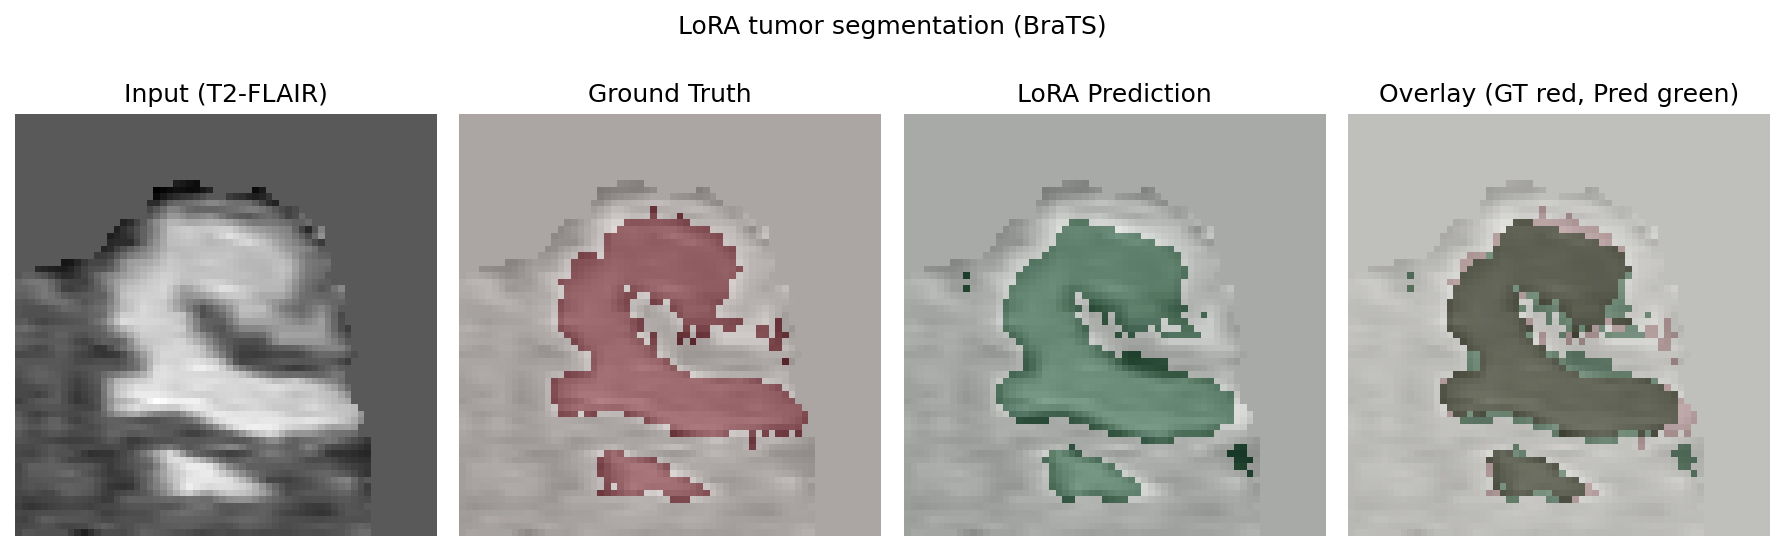
\includegraphics[width=0.7\textwidth]{figures/show_case_task2.png}
\caption{Task 1 tumor segmentation (BraTS): representative sample. Input (T2-FLAIR), Ground Truth, LoRA prediction, overlay (red=GT, green=pred).}
\label{fig:task1}
\end{figure*}

\begin{figure*}[t]
\centering
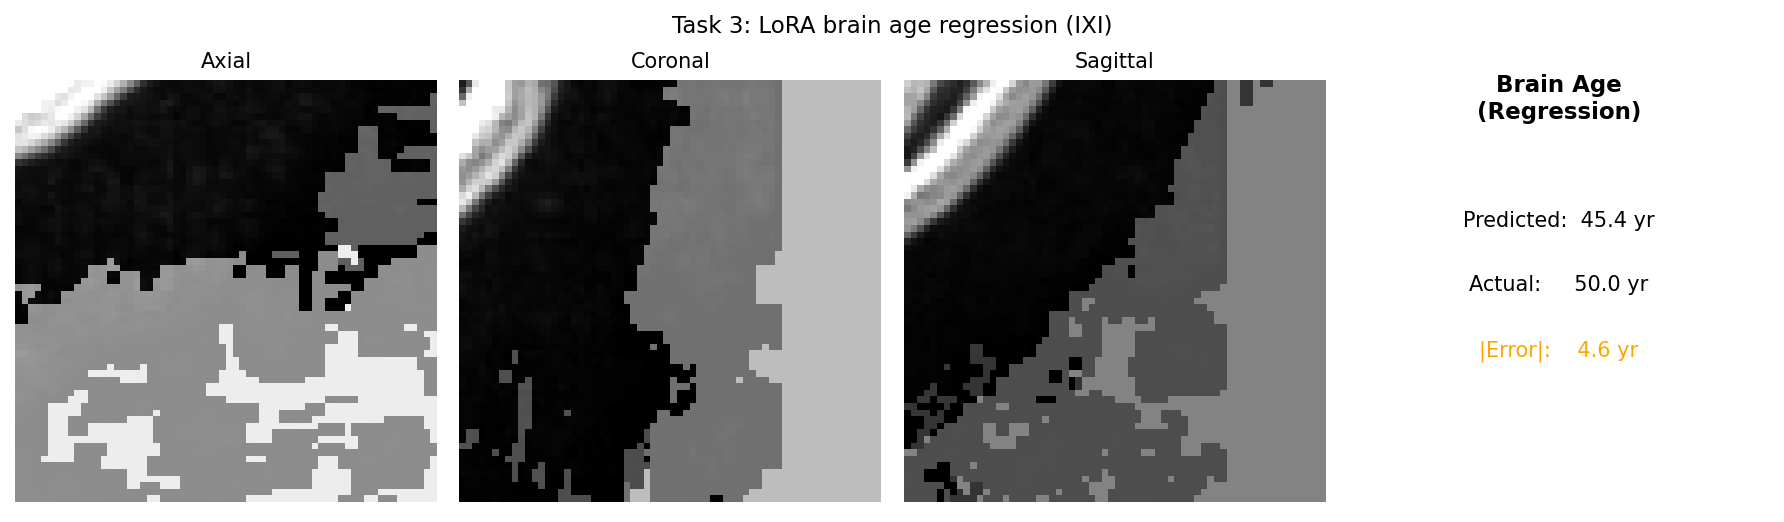
\includegraphics[width=0.7\textwidth]{figures/task3_age_s42_0.png}
\caption{Task 2 brain age regression (IXI): representative sample. Orthogonal MRI views (Axial, Coronal, Sagittal) and predicted vs.\ actual age.}
\label{fig:task2}
\end{figure*}

\begin{figure*}[t]
\centering
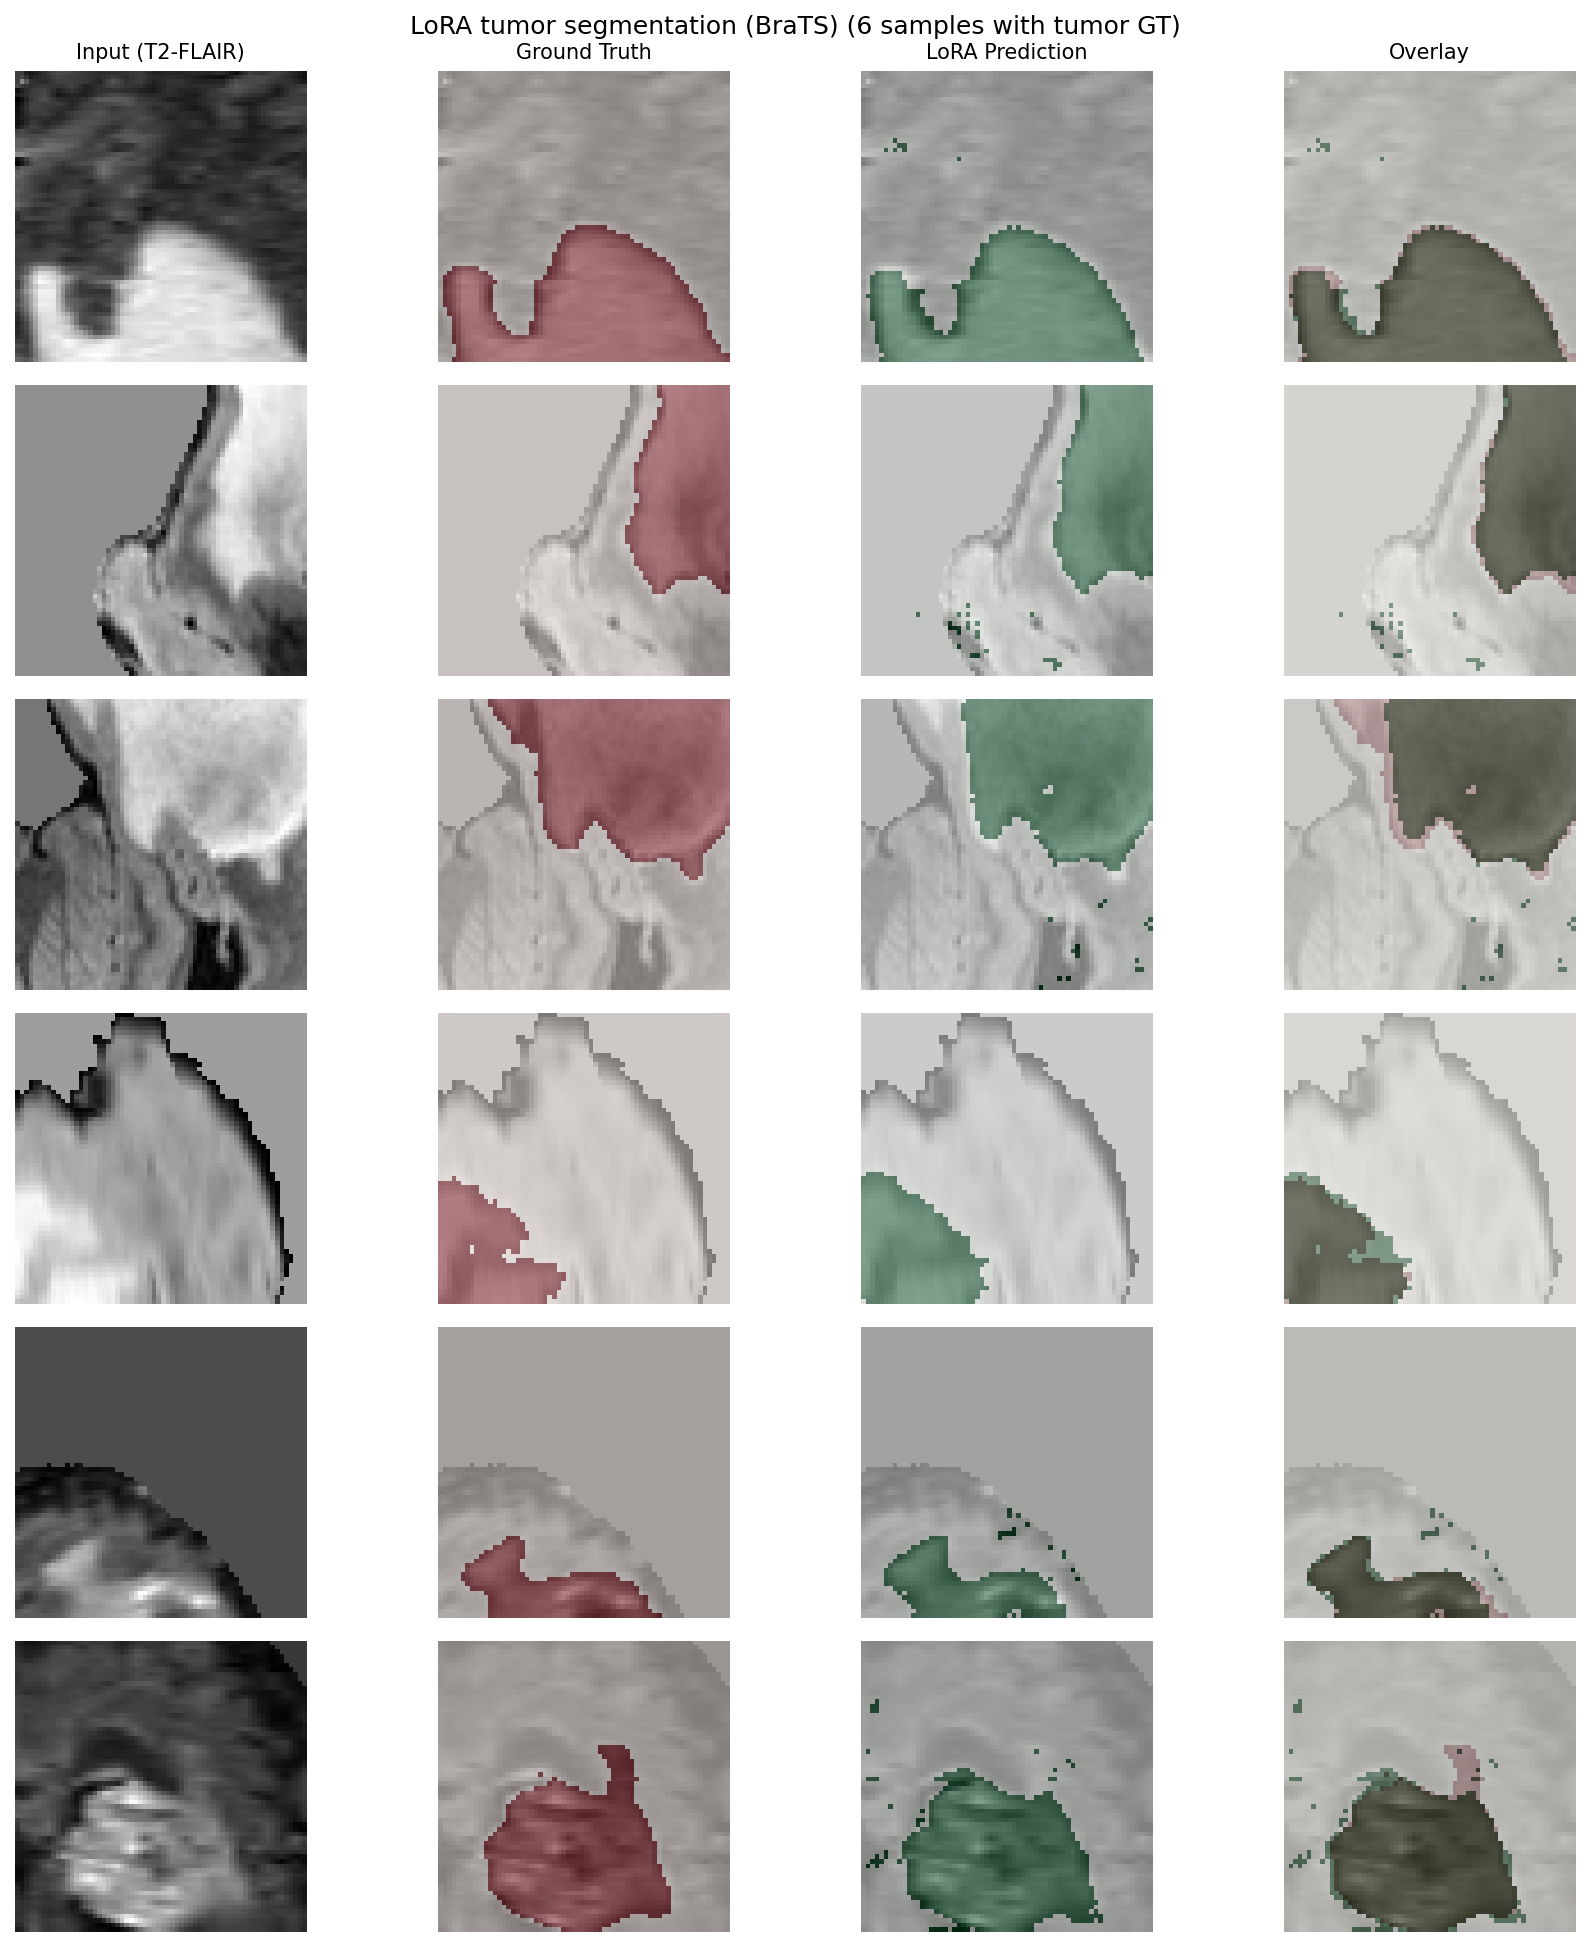
\includegraphics[width=0.85\textwidth]{figures/task2_seg_s42_stack6.png}
\caption{Task 1 tumor segmentation: six best-performing validation samples (seed 42). Each row shows input, ground truth, LoRA prediction, and overlay.}
\label{fig:app_seg_stack}
\end{figure*}

\begin{figure*}[t]
\centering
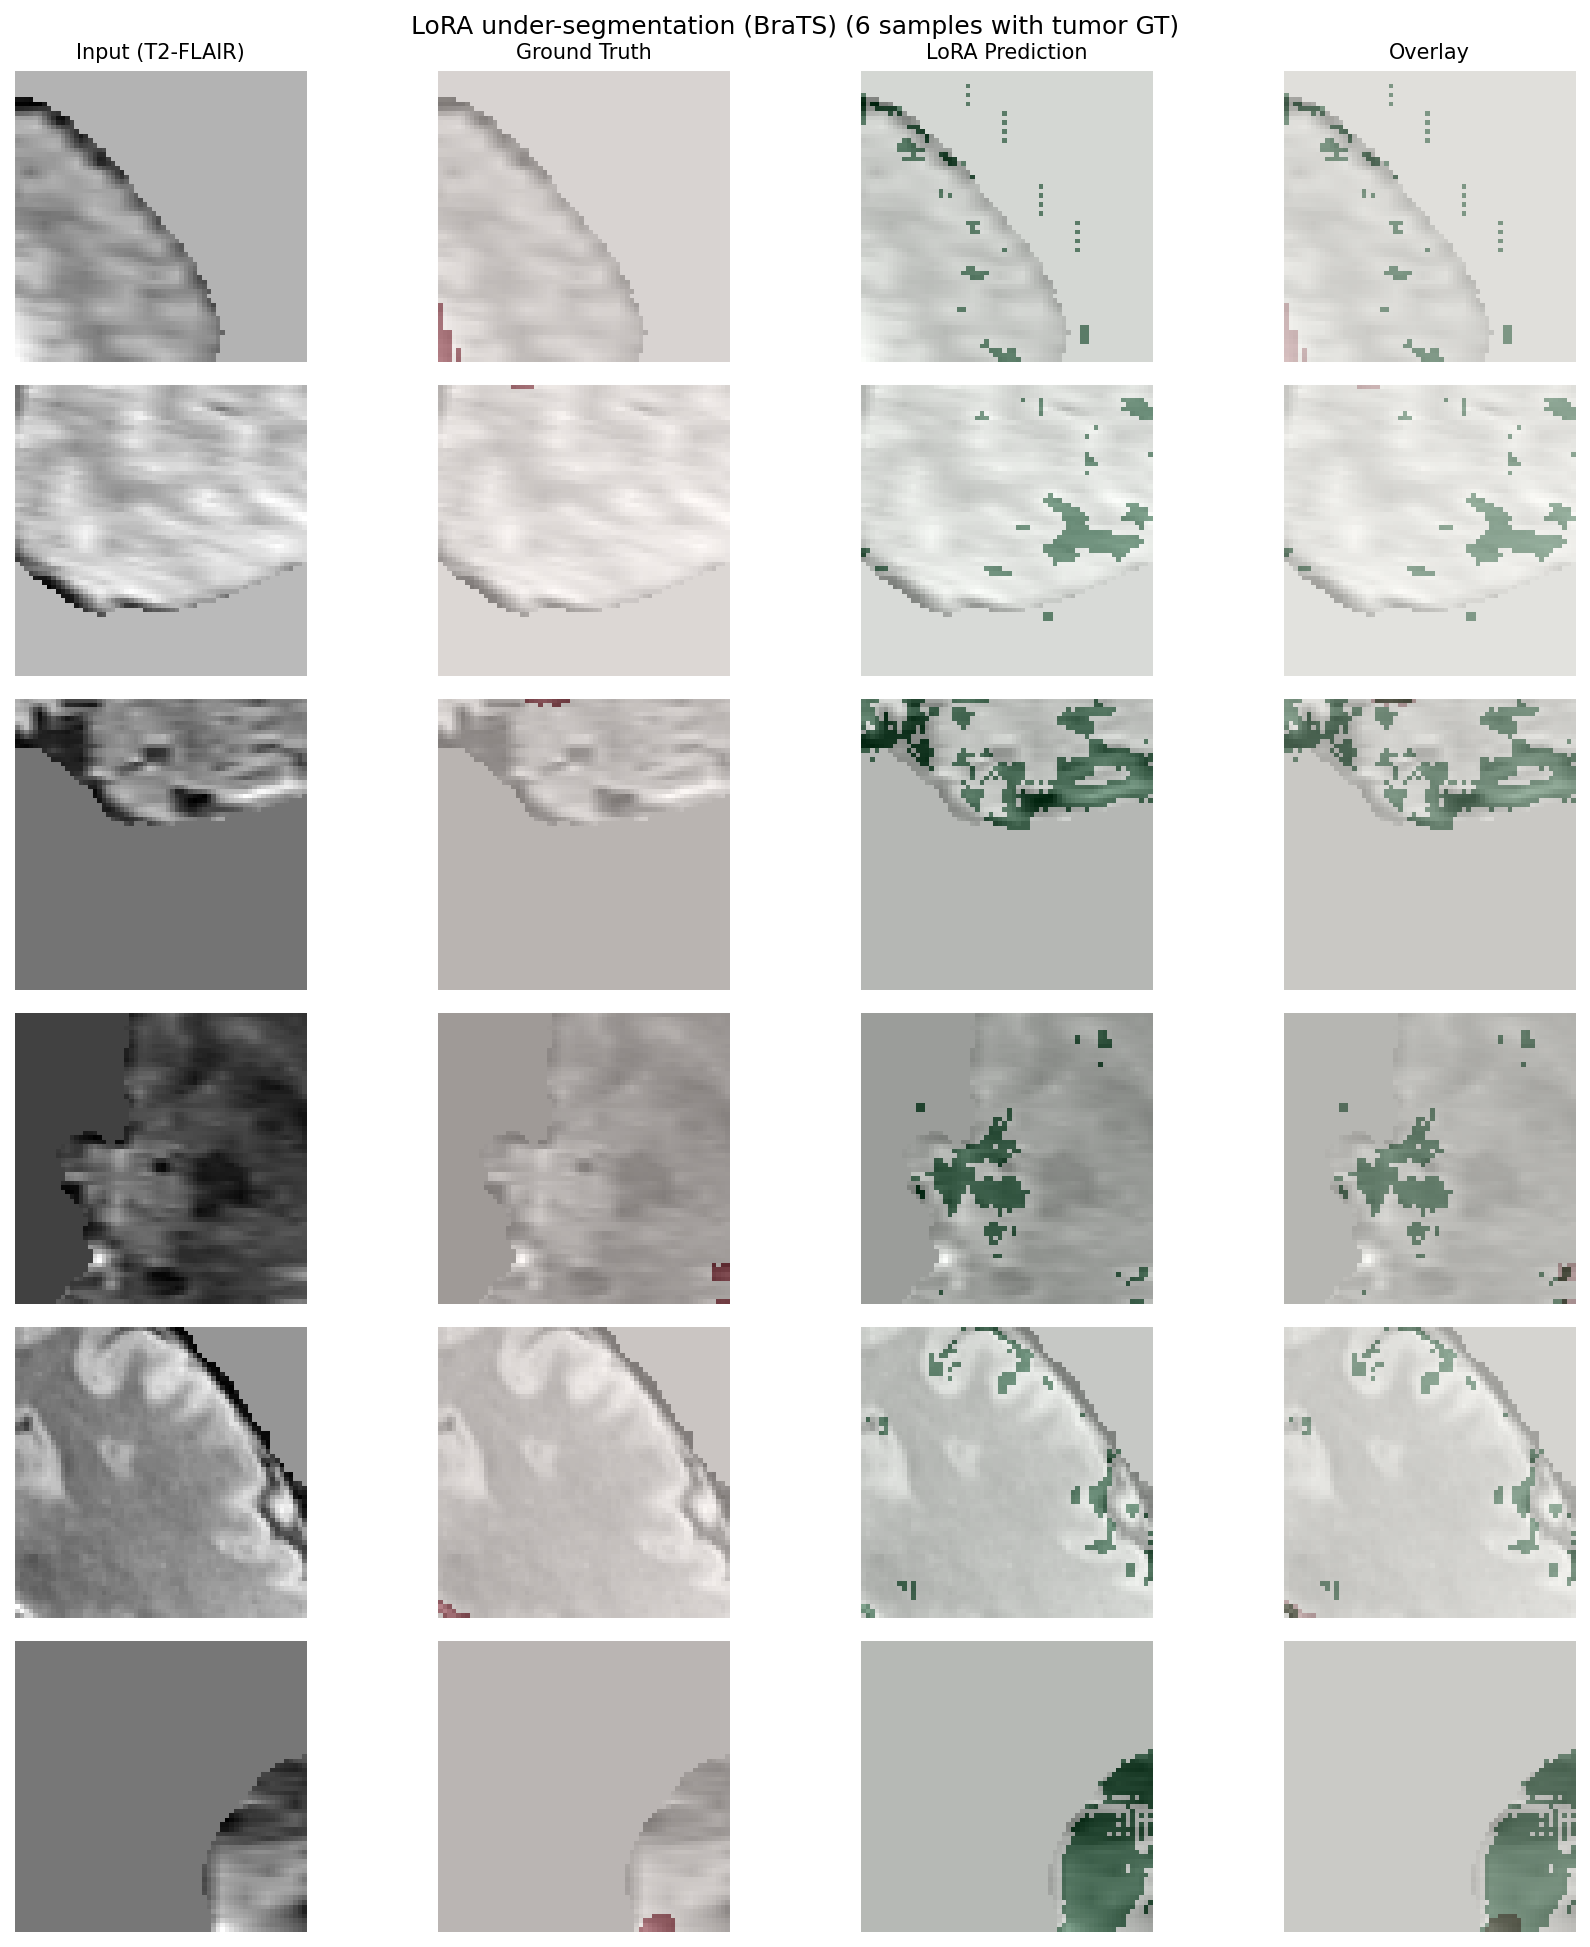
\includegraphics[width=0.85\textwidth]{figures/task2_seg_s42_stack6worst.png}
\caption{Task 1 tumor segmentation failure cases: six worst-performing validation samples (seed 42). Common failure mode: under-segmentation of tumor boundaries.}
\label{fig:app_seg_failure}
\end{figure*}

\begin{figure*}[t]
\centering
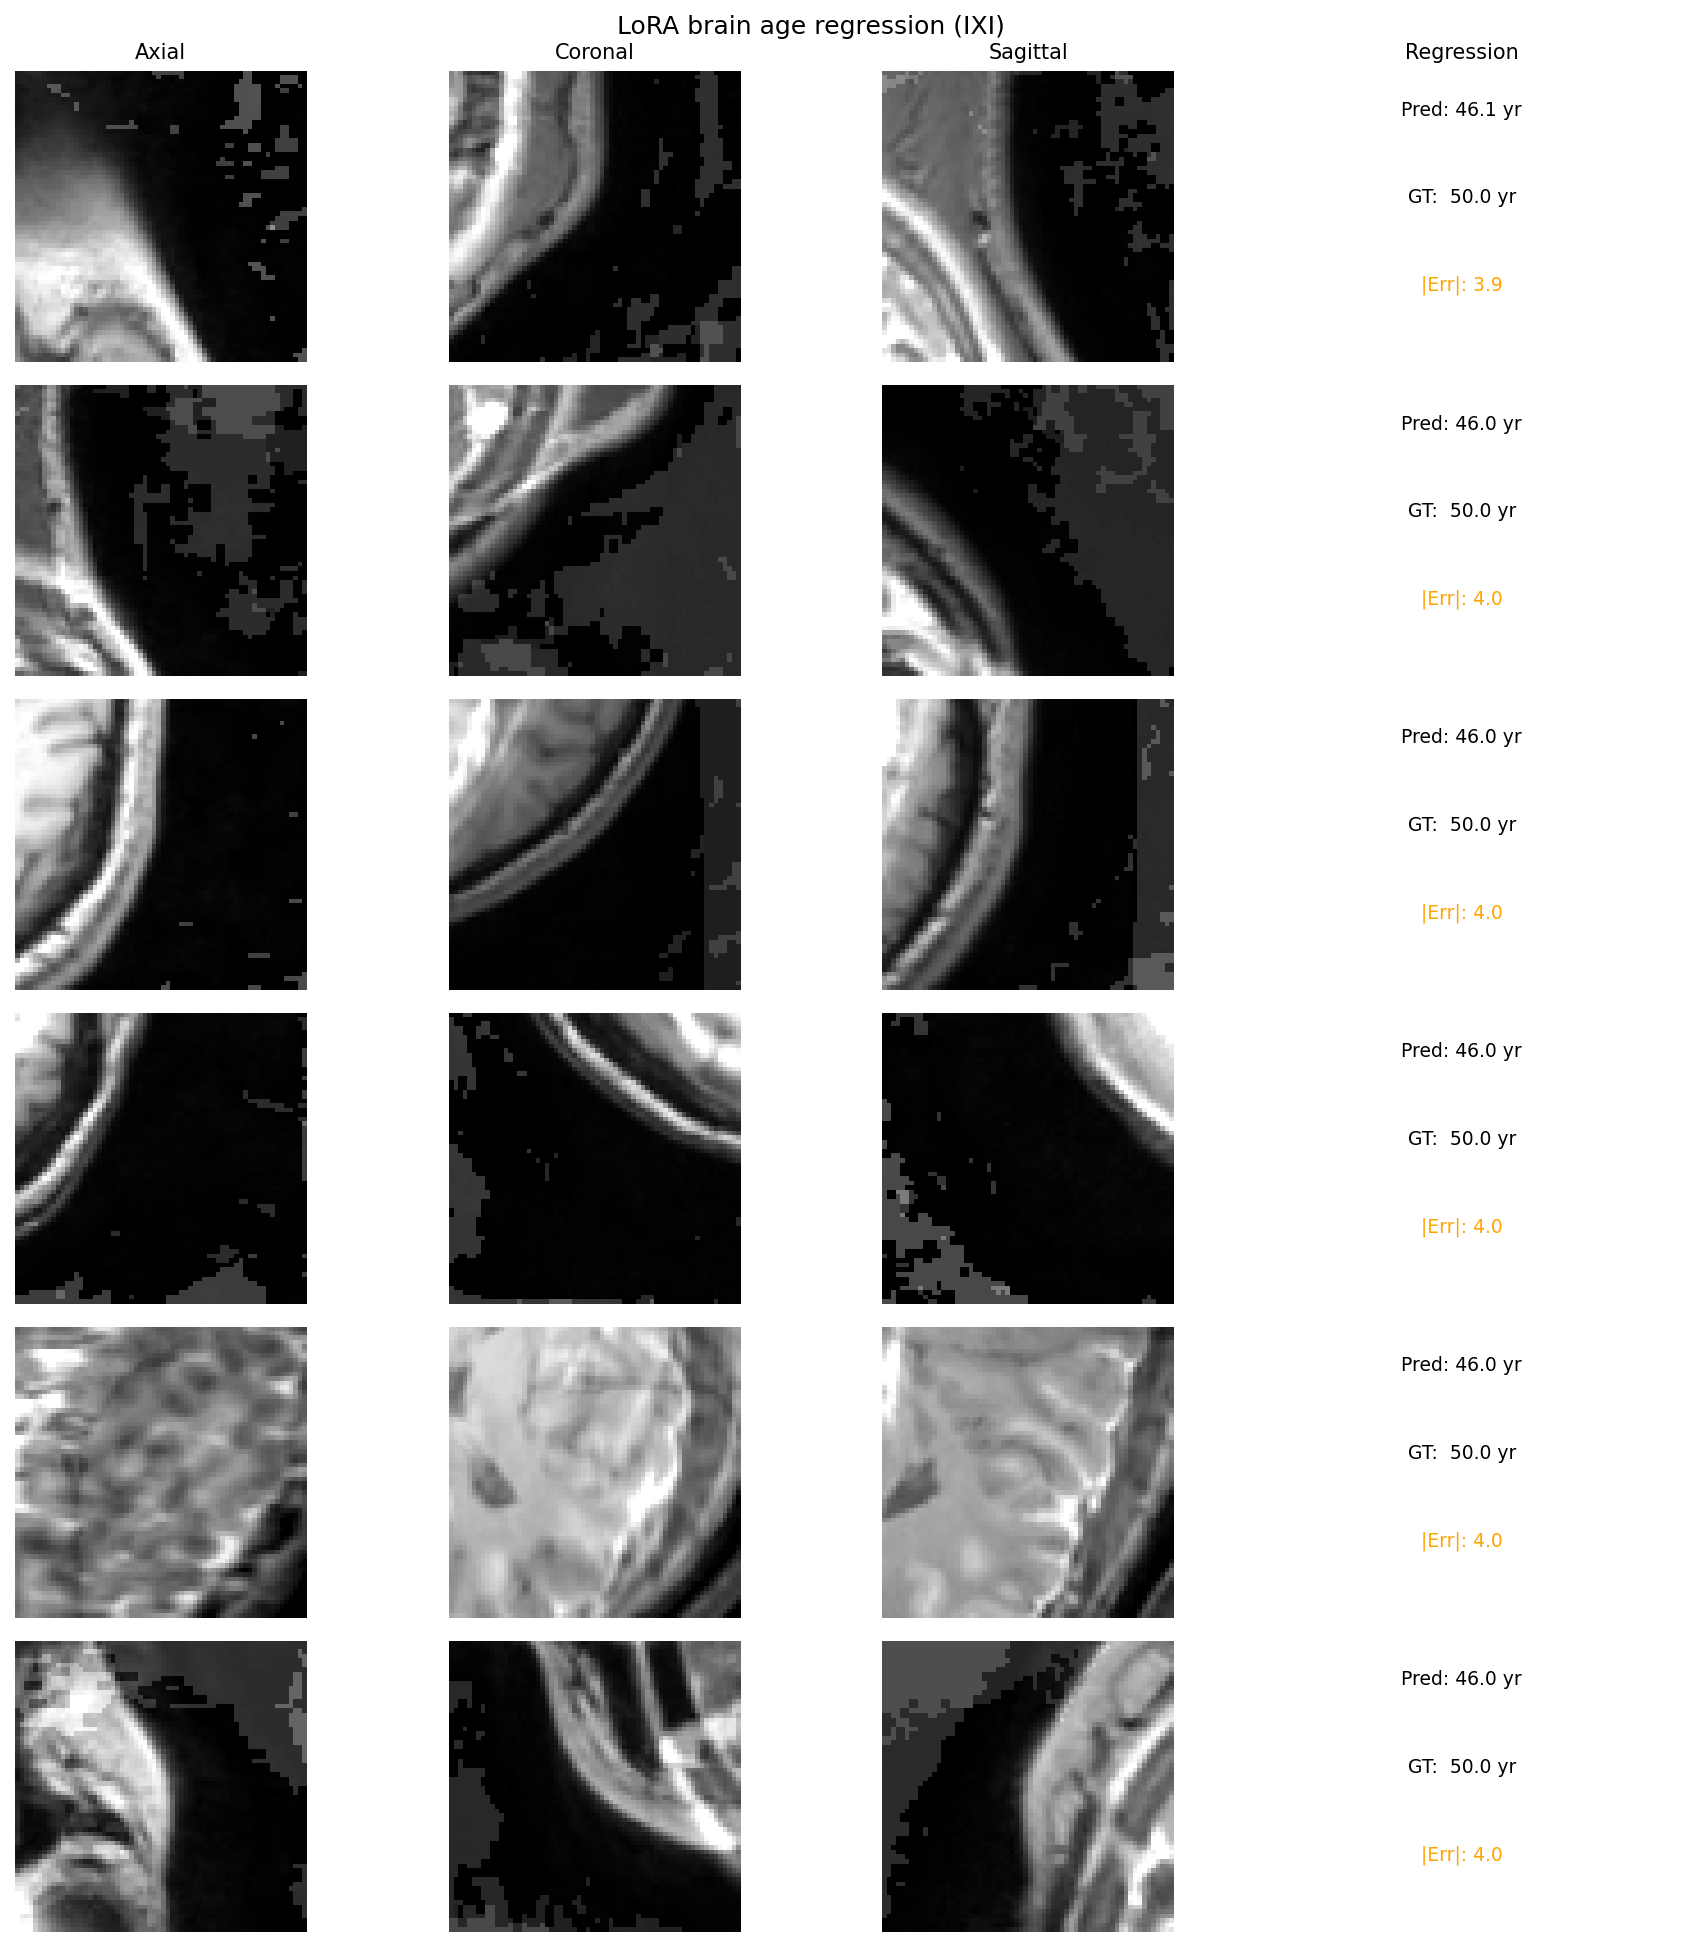
\includegraphics[width=0.85\textwidth]{figures/task3_age_s42_stack6.png}
\caption{Task 2 brain age regression: six best-performing validation samples (seed 42). Note that all six have ground-truth age 50.0\,yr, likely due to missing-age imputation in IXI metadata.}
\label{fig:app_age_stack}
\end{figure*}

\begin{figure*}[t]
\centering
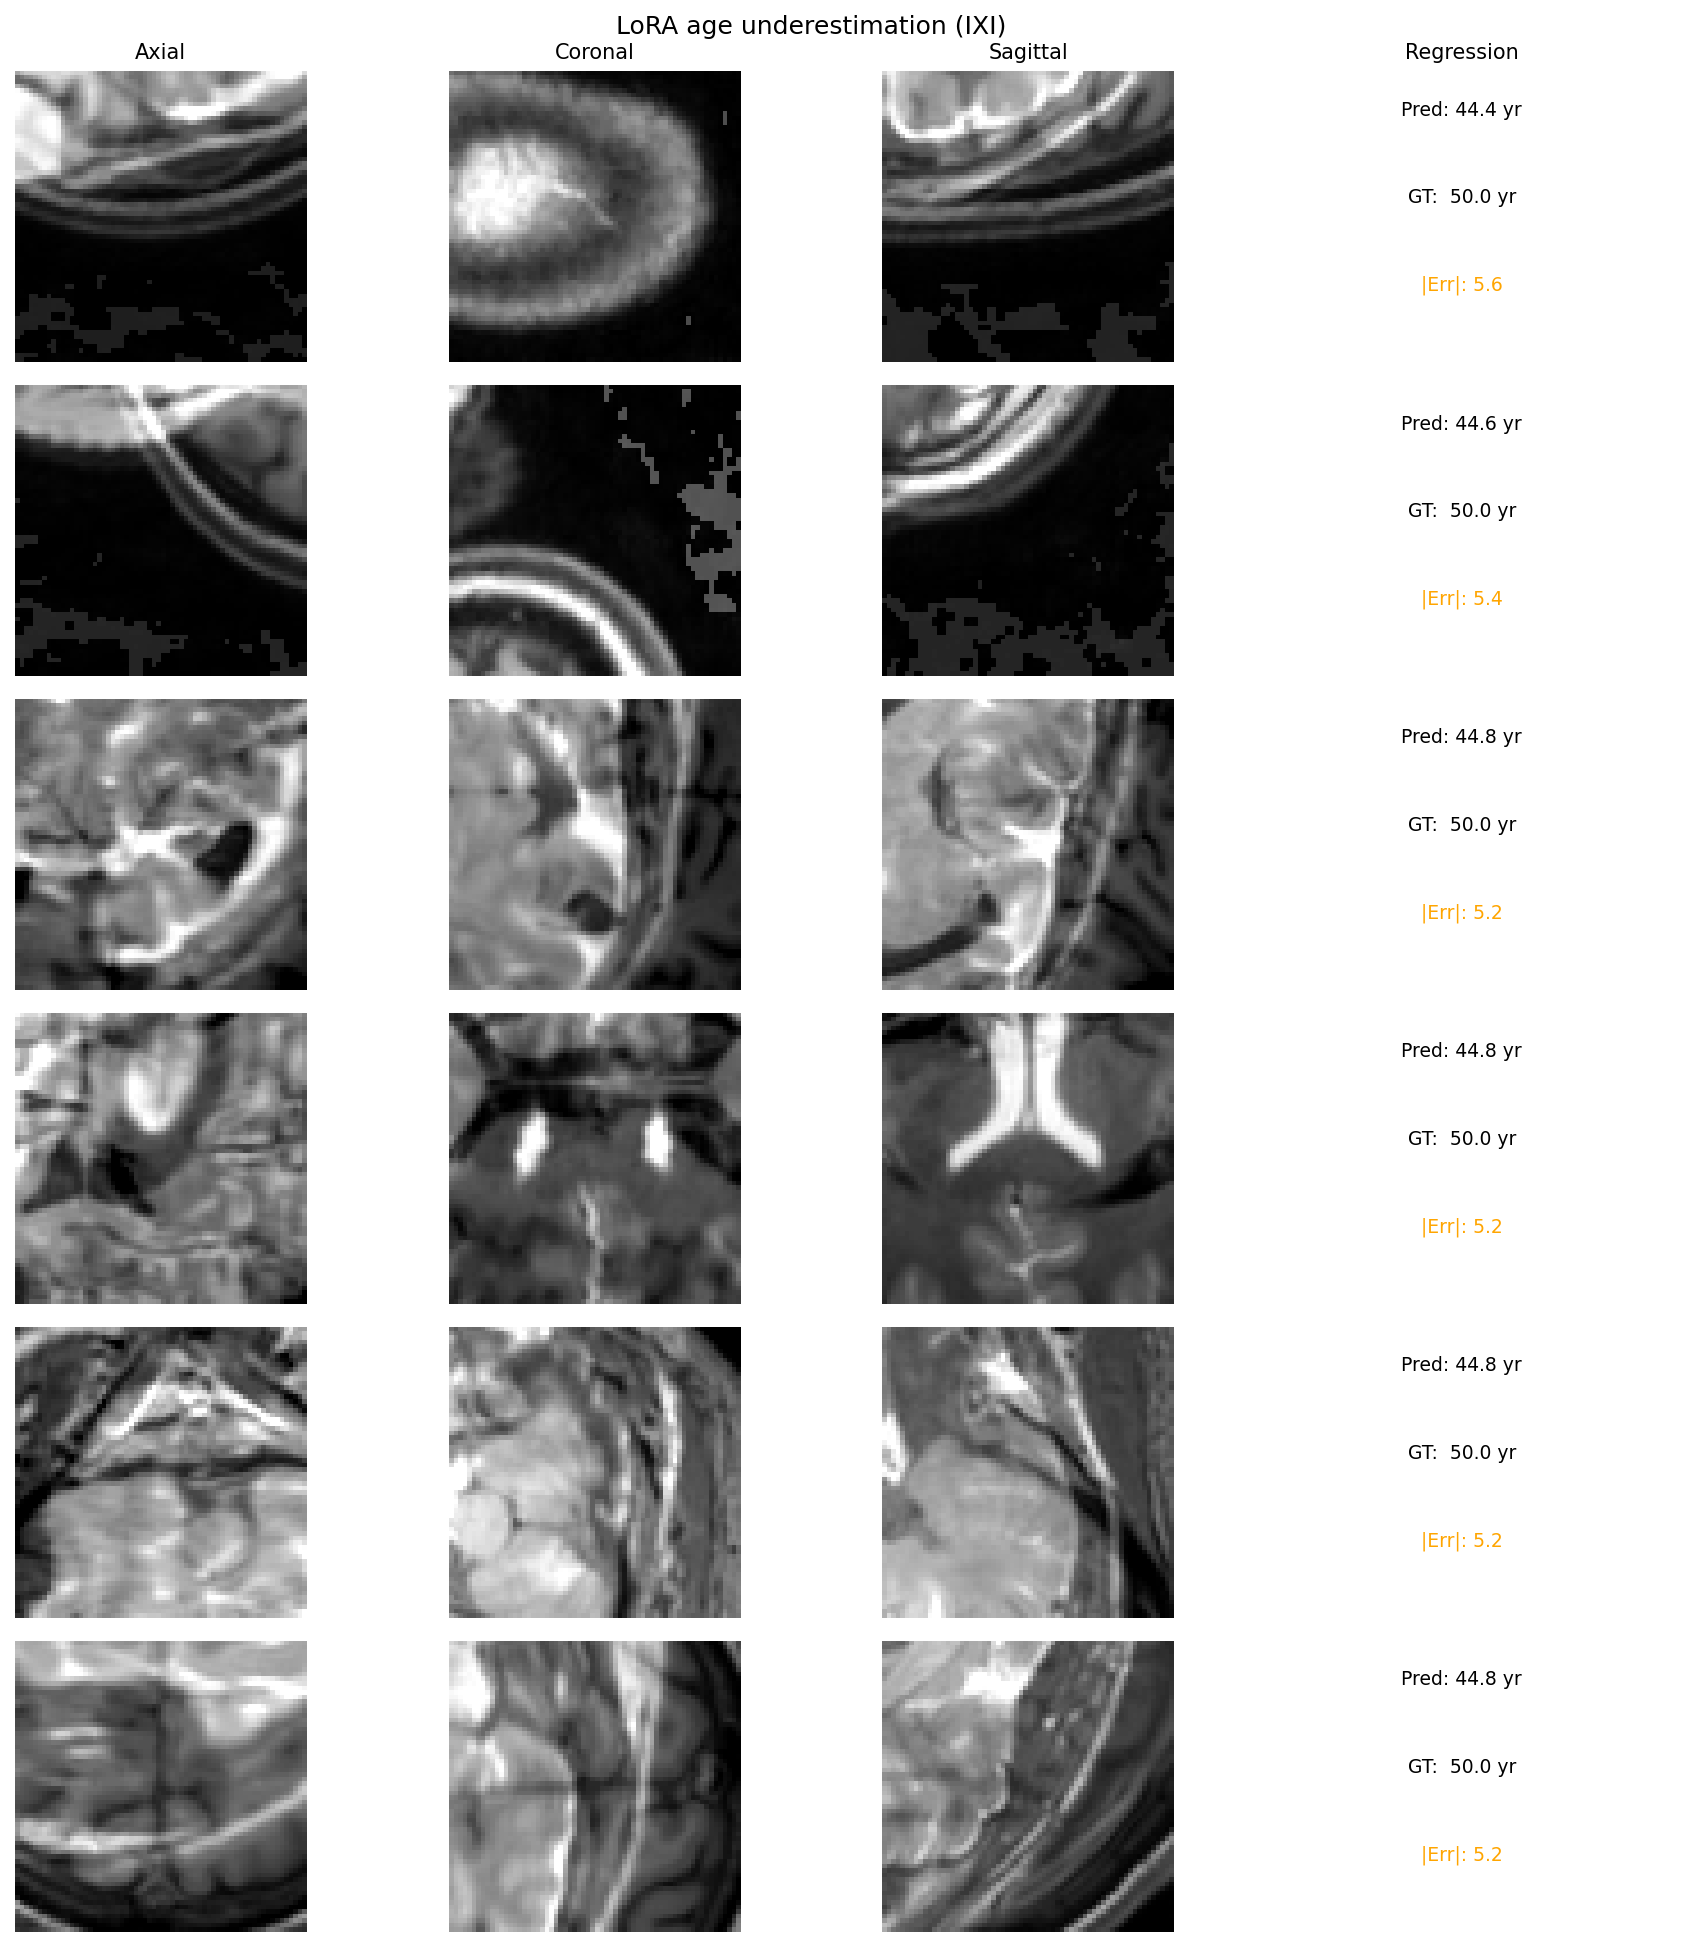
\includegraphics[width=0.85\textwidth]{figures/task3_age_s42_stack6worst.png}
\caption{Task 2 brain age regression failure cases: six worst-performing validation samples (seed 42). The model systematically underestimates brain age.}
\label{fig:app_age_failure}
\end{figure*}

\begin{table*}[t]
\caption{Extended comparison including per-task oracles (independent model per task, no continual setting). Per-task Linear uses patch=32, epochs=50. Per-task LoRA uses identical hyperparameters as continual LoRA (5 seeds). $^\dagger$Likely overfits on few-shot validation.}
\label{tab:extended}
\centering
\begin{tabular}{lcccl}
\toprule
Method & T1 Dice$\uparrow$ & T2 MAE$\downarrow$ & Setting \\
\midrule
LoRA (enc+dec) & $0.60 \pm 0.08$ & $\mathbf{0.012} \pm 0.003$ & Continual \\
EWC & $0.79 \pm 0.02$ & $0.001^\dagger \pm 0.001$ & Continual \\
LwF & $0.80 \pm 0.02$ & $0.020 \pm 0.009$ & Continual \\
Replay & $0.79 \pm 0.01$ & $0.021 \pm 0.013$ & Continual \\
Sequential Linear & $0.79 \pm 0.01$ & $1.45 \pm 0.03$ & Continual \\
Sequential FT & $0.80 \pm 0.02$ & $0.005^\dagger \pm 0.003$ & Continual (forgets) \\
\midrule
Per-task LoRA (enc+dec) & $0.58 \pm 0.09$ & $0.005 \pm 0.001$ & Oracle (no continual) \\
Per-task Linear & 0.65 & 0.063 & Oracle (no continual) \\
\bottomrule
\end{tabular}
\end{table*}

\subsection{Catastrophic Forgetting in Sequential FT}
\label{sec:forgetting}

Sequential FT achieves high T1 Dice (0.80) and very low T2 MAE (0.005) immediately after training each task. The latter likely reflects overfitting on few-shot validation. Crucially, T1 Dice after T2 training collapses to 0.16 (mean over seeds), yielding $\Delta \approx 0.64$---a clear demonstration of catastrophic forgetting when the backbone is overwritten for T2.

The forgetting pattern varies across seeds: seed 42 retains T1 Dice of 0.39 after T2, while seeds 43 and 44 collapse to near-zero (0.03 and 0.06), indicating that forgetting severity is highly stochastic in the few-shot regime. This high variance (std=0.19) makes Sequential FT unreliable for clinical deployment, where consistent performance across runs is essential.

Notably, the forgetting is asymmetric across task types. In the T2$\to$T3 order (Table~\ref{tab:main}), segmentation features are overwritten by regression training; in the reversed T3$\to$T2 order (Table~\ref{tab:t32}), regression performance collapses catastrophically (MAE rises from 0.001 to 7.17) when the backbone is subsequently fine-tuned for segmentation. This confirms that catastrophic forgetting affects both task types regardless of training order, and underscores the need for parameter-isolated approaches like LoRA.

EWC and LwF partially mitigate forgetting but remain insufficient: EWC achieves BWT$\approx$-0.65 (comparable to unregularized FT), suggesting that the diagonal Fisher approximation poorly captures parameter importance across heterogeneous tasks. LwF performs somewhat better (BWT$\approx$-0.56) but still loses over half of T1 performance. Replay, despite storing prior-task samples, shows the worst forgetting (BWT$\approx$-0.78), likely because the replay buffer is too small in the few-shot setting to adequately represent the prior task distribution.

\subsection{LoRA Ablation: Encoder-only vs Encoder+Decoder}
\label{sec:lora_ablation}

Table~\ref{tab:lora_ablation} compares LoRA placement. Encoder-only LoRA yields poor T1 Dice (0.19); encoder+decoder yields 0.50. Decoder adaptation is necessary for segmentation. T2 (regression) is similar for both.

\begin{table}[t]
\caption{LoRA placement ablation. Enc+dec = encoder+decoder.}
\label{tab:lora_ablation}
\centering
\begin{tabular}{lcc}
\toprule
LoRA Config & T1 Dice$\uparrow$ & T2 MAE$\downarrow$ \\
\midrule
Encoder-only & 0.19 & 0.20 \\
Encoder+decoder & \textbf{0.50} & 0.20 \\
\bottomrule
\end{tabular}
\end{table}

\subsection{Shot Ablation (n\_shot=16 vs 32 vs 64)}
\label{sec:shot}

Table~\ref{tab:shot} shows few-shot sensitivity for LoRA across all three shot counts. At n\_shot=16, LoRA attains T1 Dice 0.45$\pm$0.04 and T2 MAE 0.33$\pm$0.01; n\_shot=32 improves to T1 Dice 0.60$\pm$0.08 and T2 MAE 0.012$\pm$0.003; n\_shot=64 further improves T1 Dice to \textbf{0.67$\pm$0.07} while T2 MAE remains stable (0.011$\pm$0.003). The T1 Dice improvement from 32 to 64 shots (+0.07) narrows the gap with Sequential Linear (0.79), suggesting that LoRA segmentation benefits substantially from additional training samples.

Table~\ref{tab:shot64} reports the full n\_shot=64 comparison. LoRA achieves T1 Dice 0.67 with zero forgetting (BWT=0). EWC attains higher T1 Dice (0.84$\pm$0.02) but T2 MAE remains implausibly low (0.001$^\dagger$) and suffers severe forgetting (BWT$\approx$-0.77). LwF at n64: T1 Dice 0.82$\pm$0.01, T2 MAE 0.038$\pm$0.014; T1 after T2 shows high variance (0.25$\pm$0.41). The pattern is consistent with n\_shot=32: LoRA is the only method that maintains balanced performance across both tasks without forgetting.

\begin{table}[t]
\caption{Shot count ablation (LoRA enc+dec). n\_shot=16: seeds 42--43; n\_shot=32: seeds 42--44; n\_shot=64: seeds 42--46.}
\label{tab:shot}
\centering
\begin{tabular}{lcc}
\toprule
n\_shot & T1 Dice$\uparrow$ & T2 MAE$\downarrow$ \\
\midrule
16 & $0.45 \pm 0.04$ & $0.33 \pm 0.01$ \\
32 & $0.60 \pm 0.08$ & $0.012 \pm 0.003$ \\
64 & $\mathbf{0.67 \pm 0.07}$ & $\mathbf{0.011 \pm 0.003}$ \\
\bottomrule
\end{tabular}
\end{table}

\begin{table*}[t]
\caption{n\_shot=64 results. LoRA: seeds 42--46; EWC, LwF: seeds 42--44. $^\dagger$EWC T2 MAE likely overfits.}
\label{tab:shot64}
\centering
\begin{tabular}{lcccc}
\toprule
Method & T1 Dice$\uparrow$ & T2 MAE$\downarrow$ & T1 after T2 & BWT \\
\midrule
LoRA (enc+dec) & $0.67 \pm 0.07$ & $0.011 \pm 0.003$ & (=T1) & $\mathbf{0.00}$ \\
EWC & $0.84 \pm 0.02$ & $0.001^\dagger \pm 0.0003$ & $0.07 \pm 0.10$ & $-0.77 \pm 0.11$ \\
LwF & $0.82 \pm 0.01$ & $0.038 \pm 0.014$ & $0.25 \pm 0.41$ & $-0.58 \pm 0.42$ \\
\bottomrule
\end{tabular}
\end{table*}

\subsection{Phase 3 (t32\_t3t2: Task Order T3$\to$T2)}
\label{sec:t32}

Table~\ref{tab:t32} reports Phase 3 results with \textbf{task order T3$\to$T2} (regression first, then segmentation; seeds 42--44). BWT measures T3 forgetting: T2 MAE after T1 training minus T2 MAE right after T2; positive = forgetting. LoRA attains T1 Dice 0.50$\pm$0.08 and T2 MAE 0.005$\pm$0.002 with BWT=0. Sequential Linear: T1 0.78$\pm$0.01, T2 MAE 0.26$\pm$0.003; T2 after T1 = 0.36$\pm$0.05 (BWT$\approx$0.10). Sequential FT: T2 MAE 0.001$^\dagger$ right after T2, but collapses to 7.17$\pm$1.41 after T1 training (BWT$\approx$7.16)---severe catastrophic forgetting of regression when the backbone is overwritten for segmentation.

\begin{table*}[t]
\caption{Phase 3 (t32\_t3t2, T3$\to$T2 order, n\_shot=32). BWT = T2 MAE after T1 minus T2 MAE after T2 (positive = T3 forgetting). $^\dagger$Seq FT T2 MAE likely overfits.}
\label{tab:t32}
\centering
\begin{tabular}{lcccc}
\toprule
Method & T1 Dice$\uparrow$ & T2 MAE$\downarrow$ & T2 after T1 & BWT \\
\midrule
LoRA (enc+dec) & $0.50 \pm 0.08$ & $0.005 \pm 0.002$ & --- & $\mathbf{0.00}$ \\
Sequential Linear & $0.78 \pm 0.01$ & $0.26 \pm 0.003$ & $0.36 \pm 0.05$ & $0.10 \pm 0.05$ \\
Sequential FT & $0.81 \pm 0.01$ & $0.001^\dagger \pm 0.0003$ & $7.17 \pm 1.41$ & $7.16 \pm 1.41$ \\
\bottomrule
\end{tabular}
\end{table*}

\subsection{Per-Seed Breakdown (LoRA, n\_shot=32)}
\label{sec:per_seed}

Table~\ref{tab:per_seed} reports per-seed LoRA results for reproducibility. T1 Dice ranges 0.52--0.68; T2 MAE 0.008--0.014.

\begin{table}[h!]
\caption{Per-seed LoRA results (enc+dec, n\_shot=32). Continual = sequential T1$\to$T2; Per-task = independent model per task (oracle upper bound).}
\label{tab:per_seed}
\centering
\begin{tabular}{lcccc}
\toprule
 & \multicolumn{2}{c}{Continual LoRA} & \multicolumn{2}{c}{Per-task LoRA} \\
\cmidrule(lr){2-3} \cmidrule(lr){4-5}
Seed & T1 Dice$\uparrow$ & T2 MAE$\downarrow$ & T1 Dice$\uparrow$ & T2 MAE$\downarrow$ \\
\midrule
42 & 0.523 & 0.014 & 0.505 & 0.004 \\
43 & 0.598 & 0.008 & 0.613 & 0.004 \\
44 & 0.680 & 0.012 & 0.711 & 0.003 \\
45 & --- & --- & 0.463 & 0.007 \\
46 & --- & --- & 0.619 & 0.005 \\
\midrule
Mean & $0.60 \pm 0.08$ & $0.011 \pm 0.003$ & $0.58 \pm 0.09$ & $0.005 \pm 0.001$ \\
\bottomrule
\end{tabular}
\end{table}

\subsection{Resource Usage}
\label{sec:resource}

Table~\ref{tab:resource} summarizes compute. LoRA adds $<$0.1\% trainable params per task; T1 (segmentation) uses $\sim$1.7\,GB peak GPU.

\begin{table}[h!]
\caption{Resource usage (LoRA, n\_shot=32).}
\label{tab:resource}
\centering
\begin{tabular}{lccc}
\toprule
Task & Params (trainable) & GPU peak (MB) & Time (sec) \\
\midrule
T1 (segmentation) & 46,872 & 1,670 & $\sim$4k--26k \\
T2 (regression) & 28,177 & 688 & $\sim$95--780 \\
\bottomrule
\end{tabular}
\end{table}


\section{Discussion}
\label{sec:discussion}

\subsection{Strengths}
\label{sec:strengths}

Our approach offers several advantages for clinical deployment.

\textbf{Zero forgetting by construction, with no continual overhead.} Unlike regularization-based methods (EWC, SI) that only \emph{approximate} parameter importance and can still degrade prior-task performance, adapter isolation provides a \emph{hard guarantee}: BWT is identically zero because prior adapters and the backbone are never modified. This is particularly important for heterogeneous task combinations (segmentation + regression), where the loss landscapes differ fundamentally and regularization trade-offs are difficult to tune. In contrast, EWC and LwF showed BWT values of $-0.65$ and $-0.56$ respectively in our experiments, demonstrating that soft constraints are insufficient for cross-task continual learning. Importantly, the per-task LoRA oracle (Table~\ref{tab:per_seed}) confirms that the continual setting imposes \emph{no measurable cost}: continual LoRA T1 Dice ($0.60 \pm 0.08$) matches per-task LoRA ($0.58 \pm 0.09$), validating that adapter isolation fully preserves individual task performance without requiring independent model management.

\textbf{Parameter efficiency and storage.} Each LoRA adapter adds $<$0.1\% parameters relative to the backbone ($\sim$47K for segmentation, $\sim$28K for regression, vs.\ $\sim$50M backbone parameters). For $K$ tasks, total storage scales as $|\theta| + K \cdot |\phi|$, where $|\phi| \ll |\theta|$. In practice, each adapter occupies $<$200\,KB on disk, enabling deployment on resource-constrained clinical workstations. By contrast, replay-based methods require storing raw patient data from prior tasks, which may violate privacy regulations (e.g., HIPAA, GDPR).

\textbf{Modularity and scalability.} New tasks can be added without retraining or accessing prior-task data---only the new adapter and head are trained. This plug-and-play property is desirable when a clinical site incrementally adds analysis capabilities (e.g., brain age estimation after tumor segmentation) with only a small batch of newly annotated cases. The computational cost per task is also low: training T2 (regression) completes in under 13 minutes on a single RTX 3090.

\textbf{Theoretical comparison with baselines.} The key distinction between our approach and EWC/LwF lies in the nature of the forgetting prevention mechanism. EWC approximates the posterior over parameters using a diagonal Fisher information matrix, which assumes parameter independence---an assumption that breaks down for large convolutional networks. LwF relies on feature distillation, which can conflict with the new task's optimization objective. Our method sidesteps both issues by operating in a strictly \emph{orthogonal} parameter subspace per task.

\subsection{Limitations}
\label{sec:limitations}

\textbf{T1 performance gap:} LoRA (0.60 Dice) underperforms Sequential Linear (0.79) and Sequential FT (0.80) on segmentation. This may stem from LoRA capacity or decoder adaptation; ablations show encoder+decoder LoRA is necessary. \textbf{T2 systematic bias:} Wilcoxon test on brain age residuals shows significant systematic underestimation ($p<0.001$), possibly due to few-shot training, IXI demographics, and the imputation of missing ages to 50.0\,yr. \textbf{Infarct detection excluded:} The FOMO formulation includes infarct detection (ISLES 2022) as a binary classification task, but we did not evaluate it. ISLES contains mostly infarct-positive cases; a balanced classifier requires healthy (negative) controls, which ISLES does not provide. Supplementing with IXI healthy subjects would enable evaluation; we defer this to future work. \textbf{T2 MAE overfitting (Sequential FT, EWC):} Both Sequential FT (MAE 0.005) and EWC (MAE 0.001) achieve implausibly low T2 MAE; per-task linear probing on full eval achieves 0.063, suggesting these methods overfit on the few-shot validation set. We flag both in Table~\ref{tab:main}. \textbf{IXI age imputation:} Missing ages in IXI metadata are imputed to 50.0\,yr; the six ``best'' T2 samples (lowest error) in the appendix all have GT=50.0\,yr, indicating a concentration of imputed labels that limits validation interpretability. \textbf{Task order:} We evaluated T2$\to$T3 (Phase 1--2) and T3$\to$T2 (Phase 3, Table~\ref{tab:t32}). In T3$\to$T2, Sequential FT shows severe T3 forgetting (BWT$\approx$7.2); LoRA maintains BWT=0. n\_shot=64 results (EWC, LwF) are in Table~\ref{tab:shot64}.

\section{Conclusion}
\label{sec:conclusion}

We presented a few-shot continual learning framework for 3D brain MRI using frozen foundation models and task-specific LoRA adapters. In the continual T2$\to$T3 setting (tumor segmentation then brain age regression, n\_shot=32), sequential full fine-tuning suffers severe catastrophic forgetting (T1 Dice 0.80$\to$0.16, BWT$\approx$-0.65), while sequential linear probing achieves strong T1 (0.79) but fails on T2 regression (MAE 1.45). EWC attains the lowest T2 MAE (0.001) among continual methods but exhibits severe forgetting (BWT$\approx$-0.65); LwF and Replay achieve strong T1 Dice ($\sim$0.79--0.80) yet suffer moderate to severe forgetting (BWT$\approx$-0.56 to $-0.78$). Our LoRA approach achieves the best balanced performance: competitive T2 MAE (0.012$\pm$0.003) among continual methods with \textbf{zero forgetting} (BWT=0) and $<$0.1\% trainable parameters per task. Encoder+decoder LoRA is necessary for segmentation; encoder-only yields poor Dice (0.19). LoRA is the only method that simultaneously maintains competitive performance on both tasks without catastrophic forgetting. Future work will include task order ablations (T3$\to$T2) and n\_shot=64 experiments.

\bibliographystyle{IEEEtran}
\bibliography{reference}



\begin{IEEEbiography}[{
\includegraphics[width=1.1in,height=1.25in,clip,keepaspectratio]{author/chisheng.png}}]{ Chi-Sheng Chen} received a bachelor degree in Electrophysics from National Chiao Tung University and a master's degree in Biomedical Electronics and Bioinformatics from National Taiwan University. He is currently working at a financial AI startup and also serves as an AI project researcher at Harvard Medical School and Beth Israel Deaconess Medical Center. His research expertise includes time-series analysis, computer vision, brain-computer interfaces (BCI), electroencephalography (EEG), multimodal contrastive learning, and quantum machine learning. Chen has led the development of foundational models for EEG-based image generation, aiming to improve psychiatric treatment and the discovery of biomarkers for drug development. He has designed hybrid quantum-classical architectures for EEG encoding and pioneered quantum deep learning methods for contrastive learning between EEG and visual data. His research also focuses on medical speech processing and the integration of multimodal large language models (LLMs) for clinical and financial application.
\end{IEEEbiography}

\begin{IEEEbiography}[{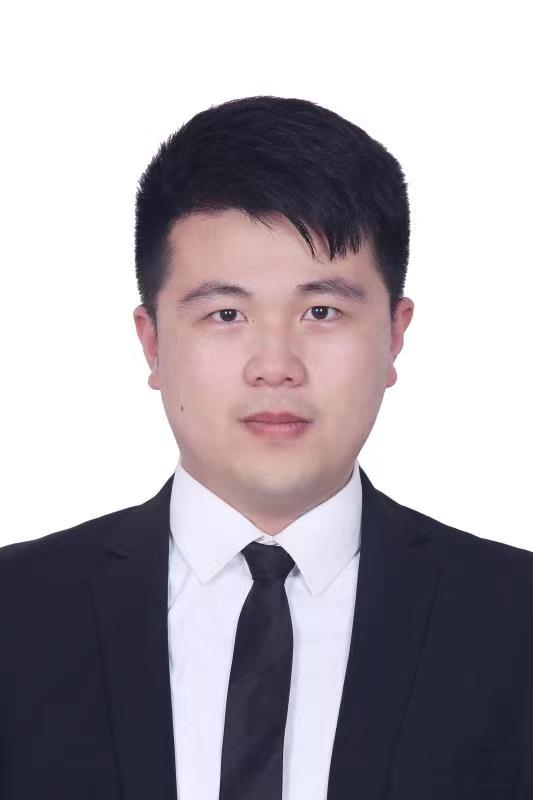
\includegraphics[width=0.9in,height=1.1in,clip,keepaspectratio]{author/Xinyu.jpg}}]{Xinyu Zhang} received the B.E. and the M.S. degree from the Information and Automatic College, Tianjin University of Science and Technology, Tianjin, China, in 2019 and 2022, separately, where he is currently pursuing the Ph.D. degree in intelligent system engineering with Luddy School of Informatics, Computing, and Engineering, Indiana University Bloomington, Bloomington, IN, USA.
His main research includes quantum neural network, deep learning, advanced signal processing, and other disciplines such as information science and large language models (LLMs).
\end{IEEEbiography}


\begin{IEEEbiography}[{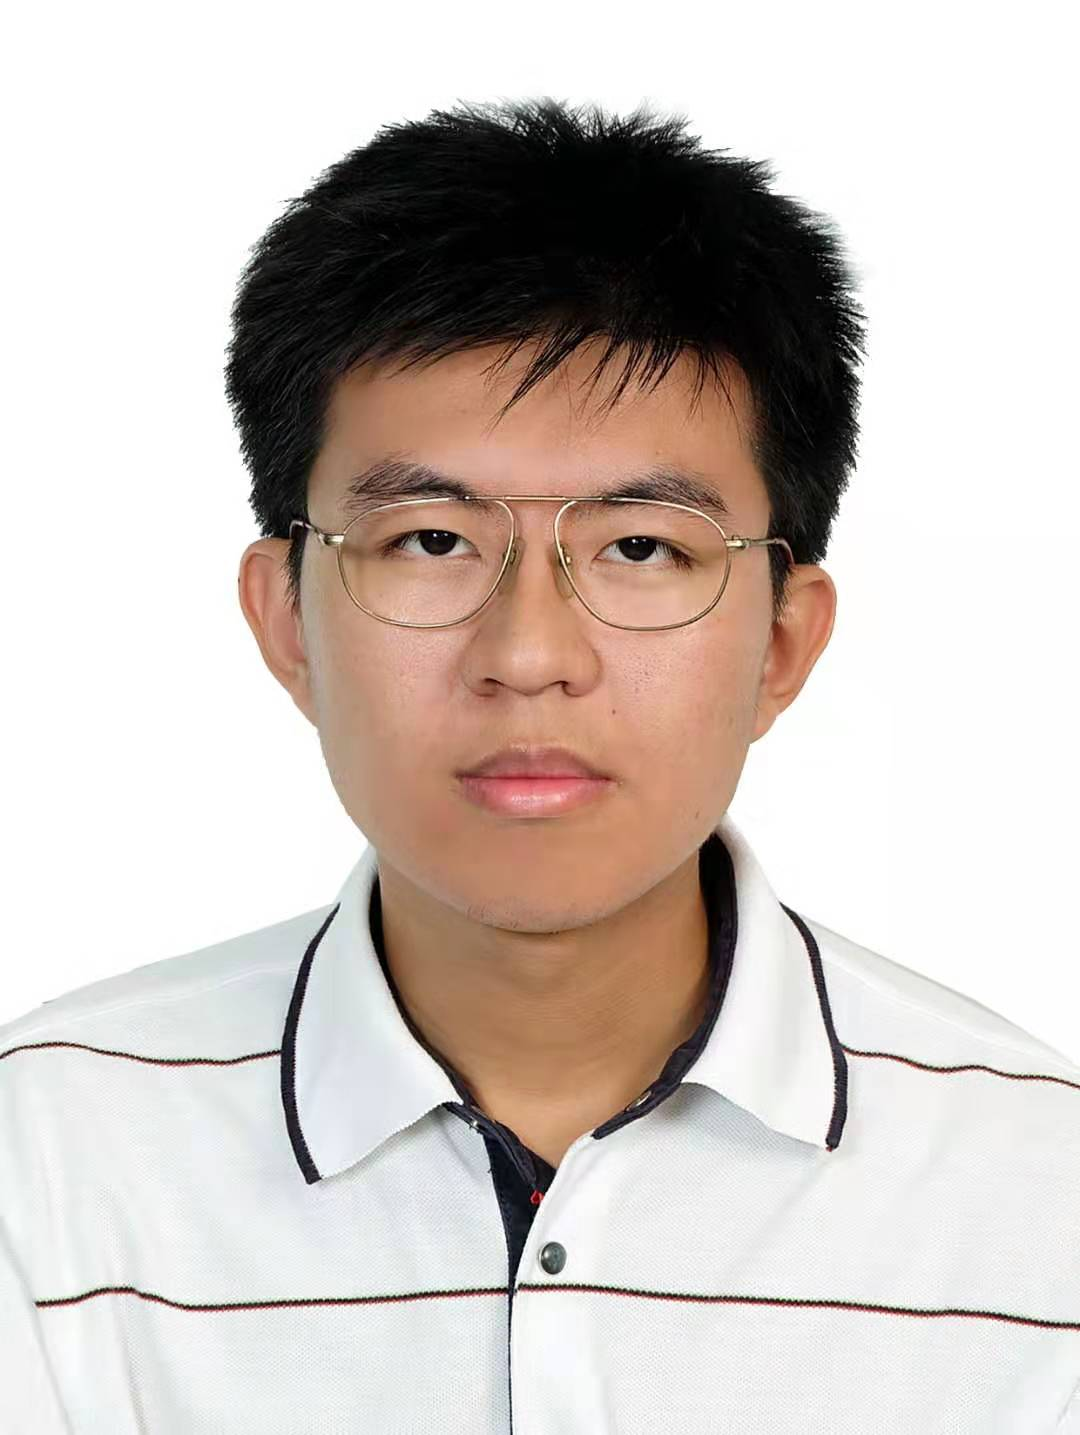
\includegraphics[width=1in,height=1.25in,clip,keepaspectratio]{author/enjui.jpg}}]{En-Jui Kuo}   received the B.S. degree in electrophysics from National Yang Ming University, Taipei, Taiwan. He then obtained his M.S. degree in physics from National Taiwan University, Taipei, Taiwan, and completed his Ph.D. in physics at the University of Maryland, USA. Currently, he is an Assistant Professor of department of electrophysics at the National Yang Ming Chiao Tung University, Taiwan.
\end{IEEEbiography}



\begin{IEEEbiography}[{
\includegraphics[width=0.9in,height=1.1in,clip,keepaspectratio]{author/Rong.jpg}}]{Rong Fu} received the B.S. degree in Communication Engineering from Jiangsu Ocean University, Jiangsu, China, in 2018, and the M.S. degree in Electronic Information Engineering from the College of Information and Automation, Tianjin University of Science and Technology, Tianjin, China, in 2023. She is currently pursuing the Ph.D. degree in Intelligent Systems Engineering with the Luddy School of Informatics, Computing, and Engineering, Indiana University Bloomington, Bloomington, IN, USA. Her research interests include signal processing and deep learning.
\end{IEEEbiography}

\begin{IEEEbiography}[{
\includegraphics[width=0.9in,height=1.1in,clip,keepaspectratio]{author/qiuzhe.jpg}}]{Qiuzhe Xie} received a bachelor's degree in Electrical Engineering from Hefei University of Technology and a master's degree in Electronics Engineering from National Cheng Kung University, followed by a Ph.D. in Electronics Engineering from National Taiwan University. His research expertise encompasses biosensors, advanced semiconductor processes, nanomaterials, and microfabrication techniques. He has spearheaded the development of nano-structural electrode arrays with ultra-thin dielectric stacking and leveraged quantum computing algorithms to enhance sensing precision. Furthermore, he has engineered CRISPR-based electrochemical sensors and developed innovative water purification systems for semiconductor manufacturing. Extending his work to practical application, he also focuses on the commercialization of medical devices, having validated business models for cardiosensor technologies through the NSF program.
\end{IEEEbiography}

\begin{IEEEbiography}[{
\includegraphics[width=0.9in,height=1.1in,clip,keepaspectratio]{author/fan.jpg}}]{Fan Zhang} received the B.S. degree in Statistics from Beijing Normal University, Beijing, China, in 2016, the M.S. degree in statistics from National Cheng Kung University, Taiwan, in 2018, and the Ph.D. degree in statistics from Arizona State University, Tempe, AZ, USA, in 2024. She is currently an Assistant Professor with the Department of Mathematics, Boise State University, Boise, ID, USA. Her research interests include design and analysis of experiments, variable selection, uncertainty quantification, Bayesian modeling and inference, and quantum-enhanced machine learning.

\end{IEEEbiography}


\end{document}
